\documentclass[preprint,12pt,times,a4paper]{elsarticle}

\usepackage{graphicx}
\usepackage{amssymb}
\usepackage{amsmath}
\usepackage{lineno}
\usepackage{xspace}
\usepackage{lipsum}
\usepackage{cleveref}
\usepackage{stackengine}
\usepackage{titlesec}
\usepackage{xcolor}
\usepackage[bitstream-charter]{mathdesign}
\usepackage[T1]{fontenc}
\usepackage{geometry, float}
%\usepackage{biblatex}
%\addbibresource{paper.bib}

\geometry{a4paper}

\usepackage[normalem]{ulem}
\usepackage{stackengine}

\journal{Nuclear Instruments and Methods in Physics Research A}

\newcommand{\XGB}{XGBoost}

\begin{document}

\begin{frontmatter}

\setcounter{page}{0}
\title{Simulation Study of Angular Resolution of a New Electromagnetic Sampling Calorimeter}

\author[jbnu]{Junlee~Kim}
\ead{junlee.kim@cern.ch}
%\cortext[cor1]{Corresponding author. Tel.: +82-xxxxxxxxx.}

\author[jbnu]{Eun-Joo~Kim\corref{cor1}}
\ead{ejkim@jbnu.ac.kr}
\cortext[cor1]{Corresponding author. Tel.: +82-10-4581-5649.}

\author[korea]{Young~Jun~Kim}
\author[korea]{Jung~Keun~Ahn}
\author[kek]{Gei~Youb~Lim}

\address[jbnu]{Division of Science Education, Jeonbuk National University, Jeonju 54896, Korea}
\address[korea]{Department of Physics, Korea University, Seoul 02841, Korea}
\address[kek]{Institute of Particle and Nuclear Studies (IPNS), High Energy Accelerator Research Organization (KEK), Tsukuba 305-0801, Japan}

%\date[]{Received 6 August 2007}

\begin{abstract}
We report simulation results on the angular resolution of an electromagnetic (EM) sampling calorimeter with photons being in the range of 100~MeV to 2~GeV. A simulation model of the EM calorimeter consists of alternating layers of a 1-mm-thick Pb plate and a 5-mm-thick plastic scintillator plate. The scintillator plates are alternatively segmented in horizontal and vertical strips. In this study, we obtained energy deposits in individual strips using Geant4 simulations and reconstructed incident photon angles using the XGBoost with gradient boosted decision trees. The performance of the angle reconstruction depends on both of the detector configuration and the goodness of the machine learning. The obtained angular resolution can be expressed as $0.24 \oplus 1.24/\sqrt{E_{\gamma}}$, where the $E_{\gamma}$ is incident photon energy in GeV. This energy dependence is consistent for different incident angles in the range of 15 to 40 degrees.

\end{abstract}
\begin{keyword}
% keywords here, in the form: keyword \sep keyword
Electromagnetic Calorimeter \sep Geant4 \sep XGBoost
\end{keyword}

\end{frontmatter}


\section{Motivation}
\label{sec:mot}
Electromagnetic (EM) calorimeter plays an important role in experimental studies of nuclear and particle physics~\cite{KOTO:MB, CMS:EMCAL, BELLE:EMCAL}. Recently, sampling calorimeters that consist of alternating layers of an absorber generating EM showers and an active medium providing signals have become popular especially in large-scale high energy experiments. In sampling calorimeters, energy deposited in the active medium fluctuates because the active layers are interleaved with absorber layers. This so-called sampling fluctuation dominates the energy resolution. This sampling fluctuation can be improved by optimizing the thickness ratio of the absorber to the active medium. A 3-m-long cylindrical calorimeter constructed of alternating layers of Pb and plastic scintillator plates is an example of a sampling calorimeter~\cite{Murayama:2020mcp}.

In addition to the alternating layer structure, the segmented structure of the active medium facilitates the measurement of lateral distributions of the EM shower along the incident photon direction. Energy deposits in the active medium segmented in both the longitudinal and lateral directions allow the incident direction of the incoming photon can be deduced. A limitation in angular resolution, especially for low energy photons, results from the stochastic behaviors of the EM shower development~\cite{trk:ref}. We have performed a simulation study to deduce the incident angle of photon, which will be a starting point to design a detector configuration to provide precise angle measurement for photons.

This paper describes a machine learning approach based on XGBoost (XGB) which is an optimized distributed gradient boosting library~\cite{xgboost:2016}. With the machine learning algorithms under the Gradient Boosting framework, we can deduce the direction of incident photons entering a sampling calorimeter with alternating layers of a Pb plate and plastic scintillator strips in horizontal and vertical directions.

\section{Electromagnetic Shower Simulation}
\label{sec:ems}

\begin{figure}[!hbt]
\centering
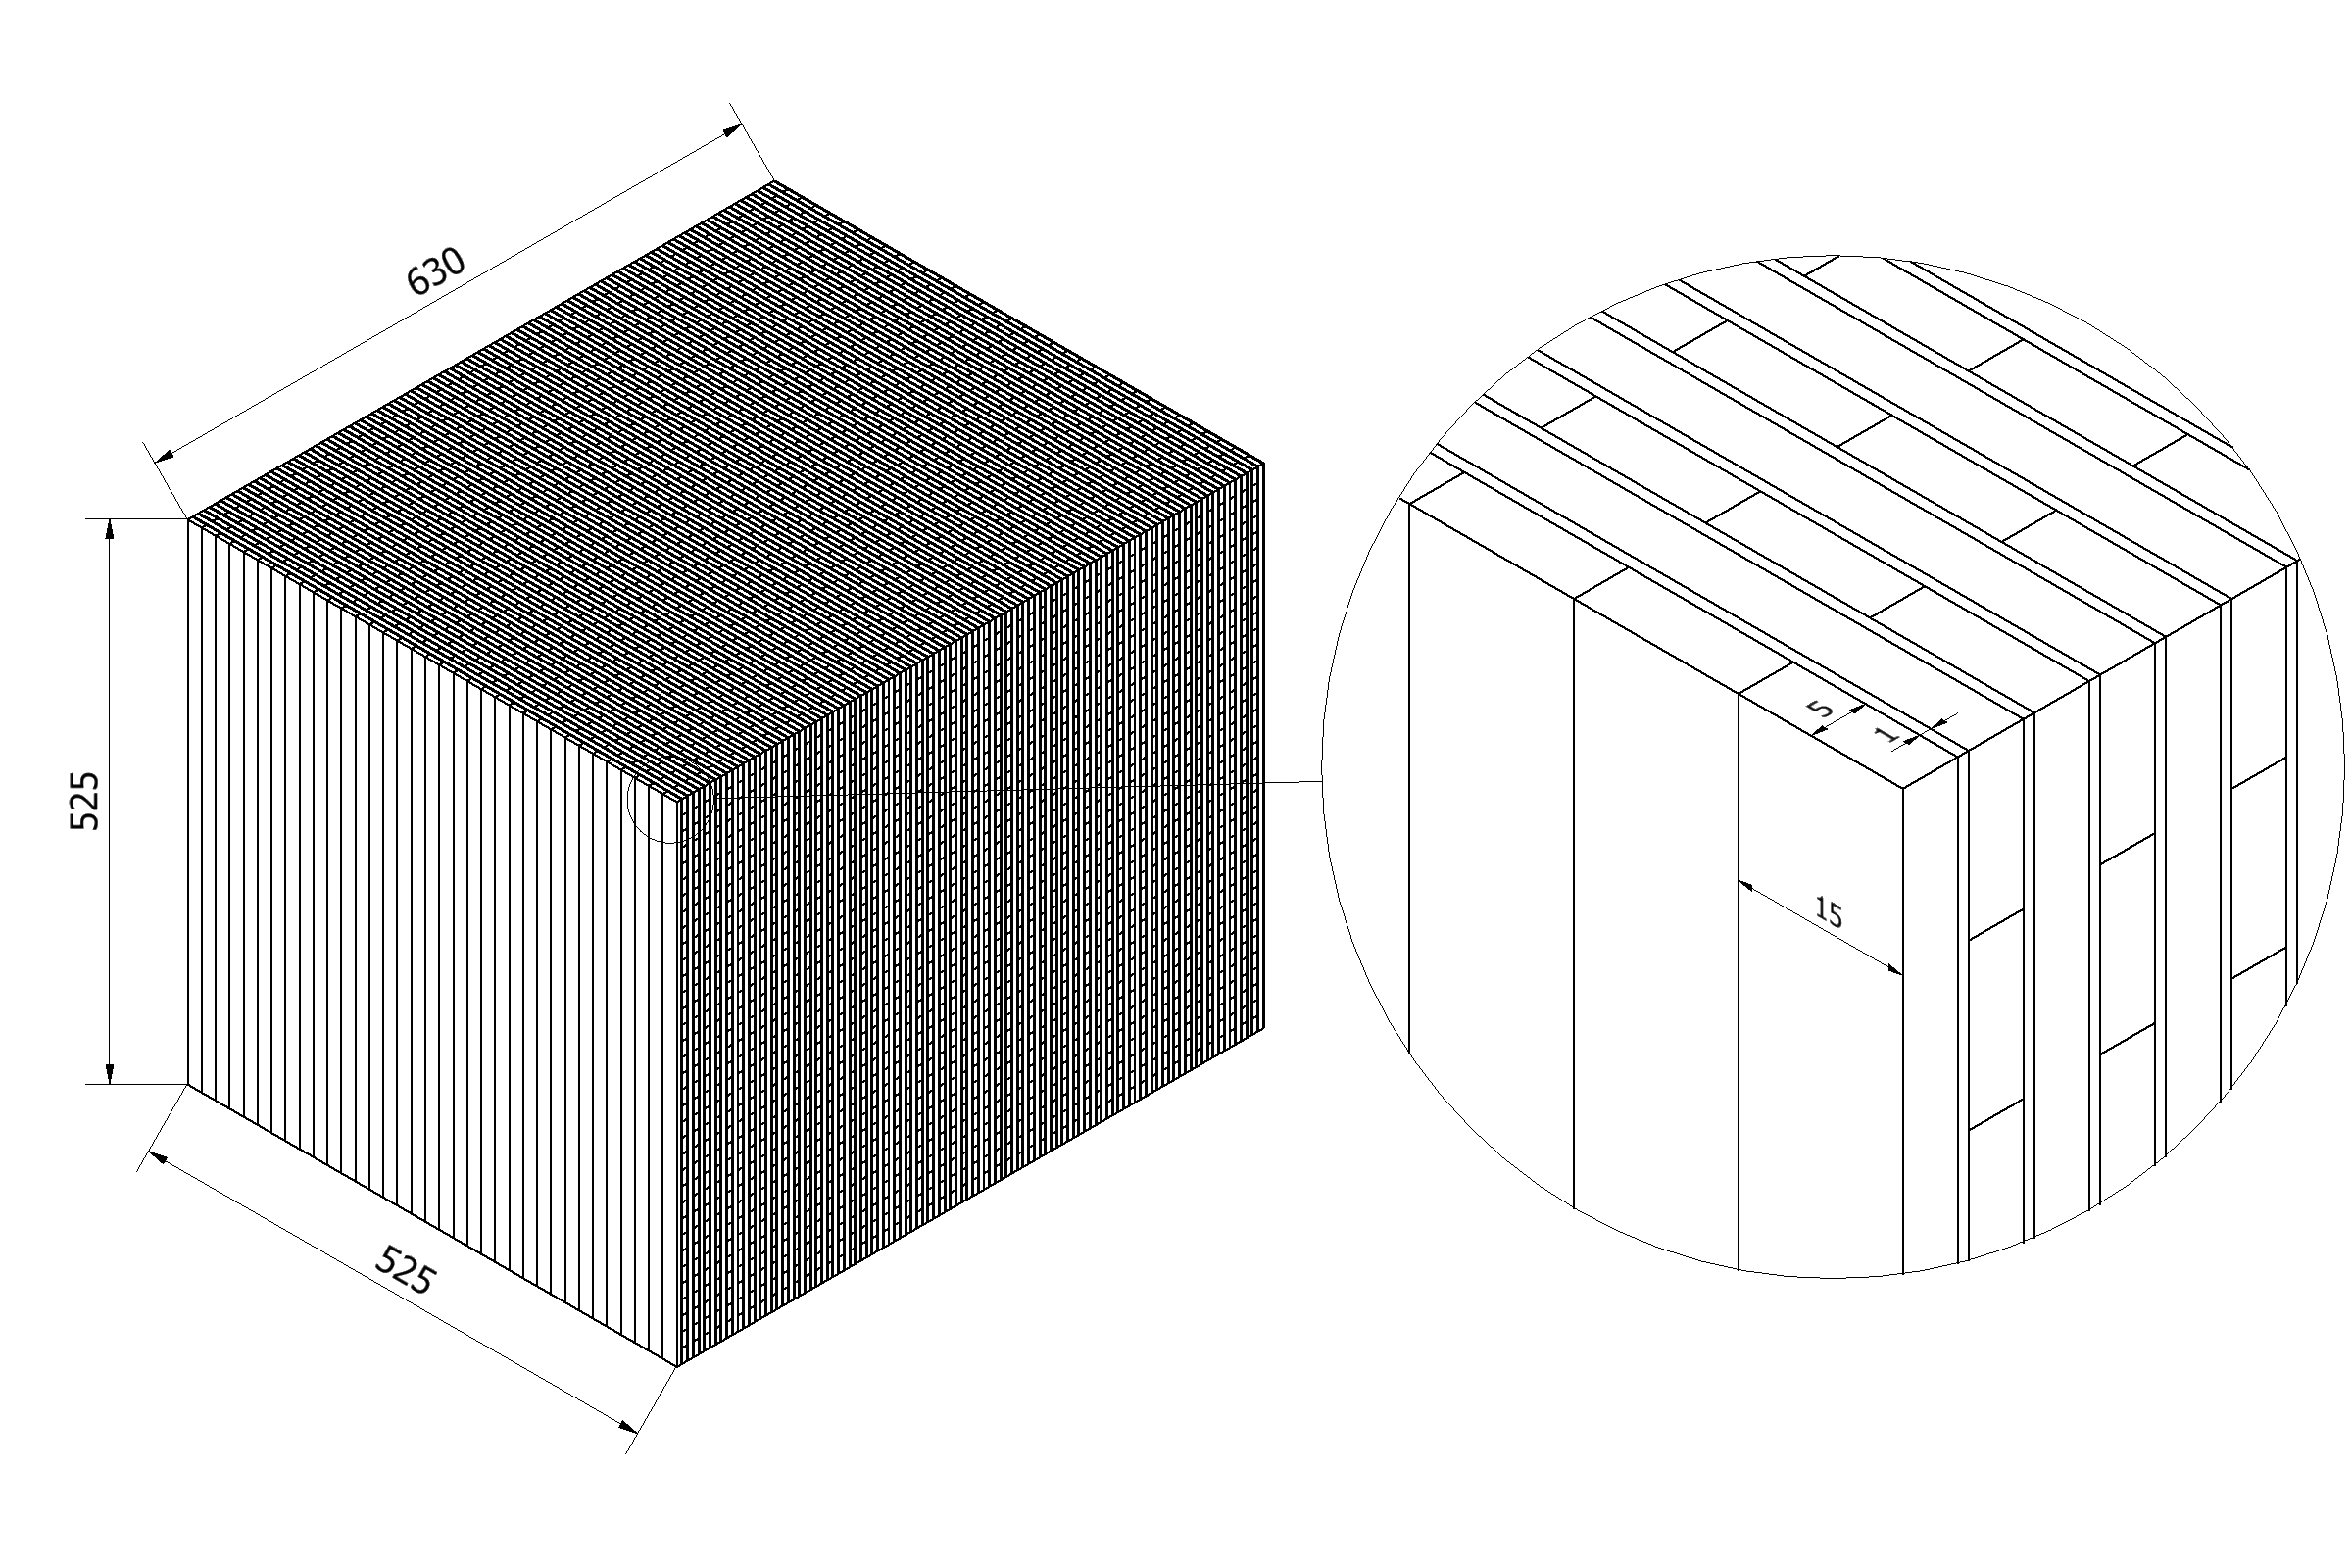
\includegraphics[width=0.6\textwidth]{figures/Fig1_detector_schematic.jpeg}
\caption{ Schematic of the sampling calorimeter model consisting of 105 alternating layers of a Pb plate and a segmented scintillator plate in 35 strips. Each scintillator plate is oriented alternatively in horizontal and vertical directions. See text for details. }
\label{fig:det_conf}
\end{figure}


The sampling calorimeter was designed as a block consisting of alternating layers of a 1-mm-thick Pb absorber and a 5-mm-thick polyvinyltoluene-based plastic scintillator. The plastic scintillator is segmented in 15-mm-wide strips, which are alternatively oriented in the vertical and horizontal directions as shown in Fig.~\ref{fig:det_conf}. It has a cross-section of 525~$\times$~525~mm$^{2}$ and accommodates 105 alternating layers of 630~mm length, which corresponds to 20 radiation length (20$X_{0}$) that is sufficiently long to absorb full photon energy in the range of 0.1 to 2~GeV.

\begin{figure}[!hbt]
\centering
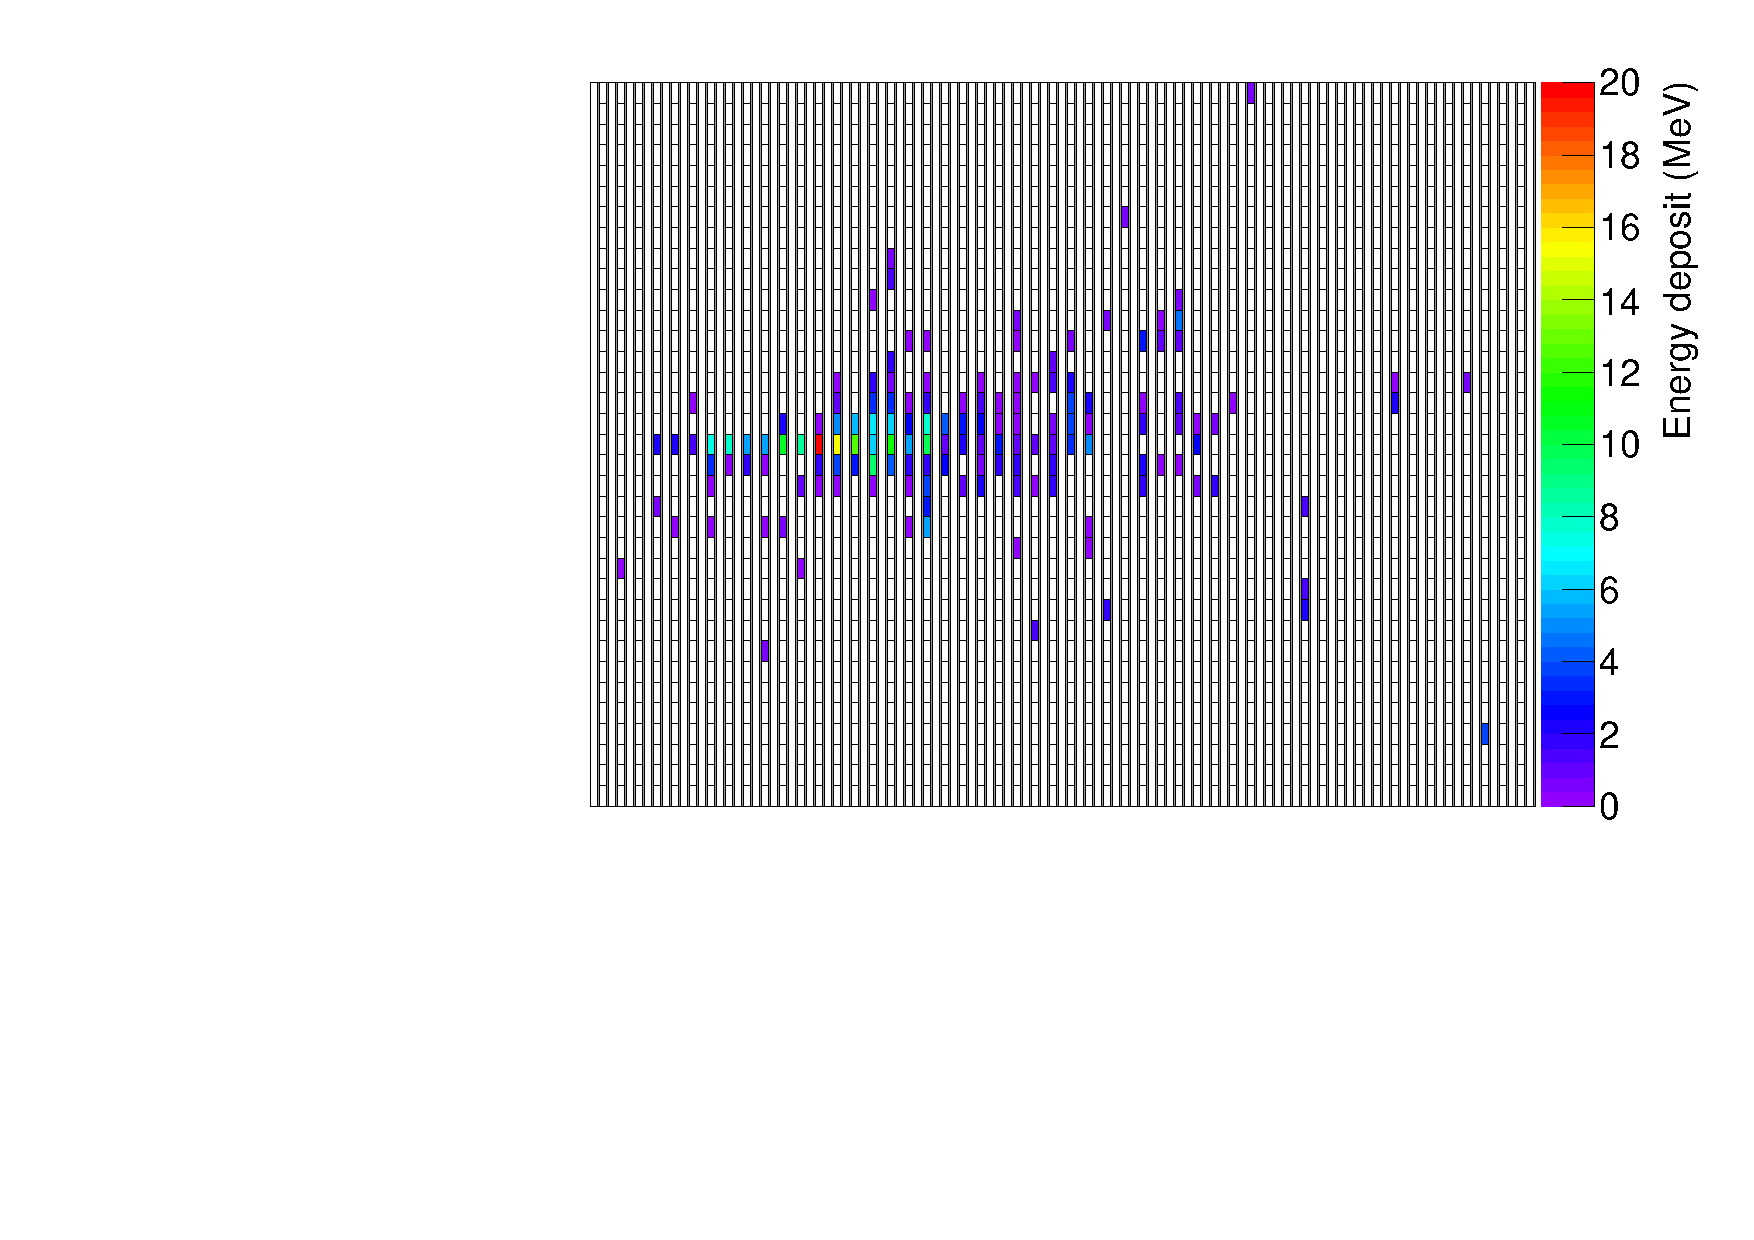
\includegraphics[width=0.48\textwidth]{figures/Fig2_EMShower_XZ.pdf}
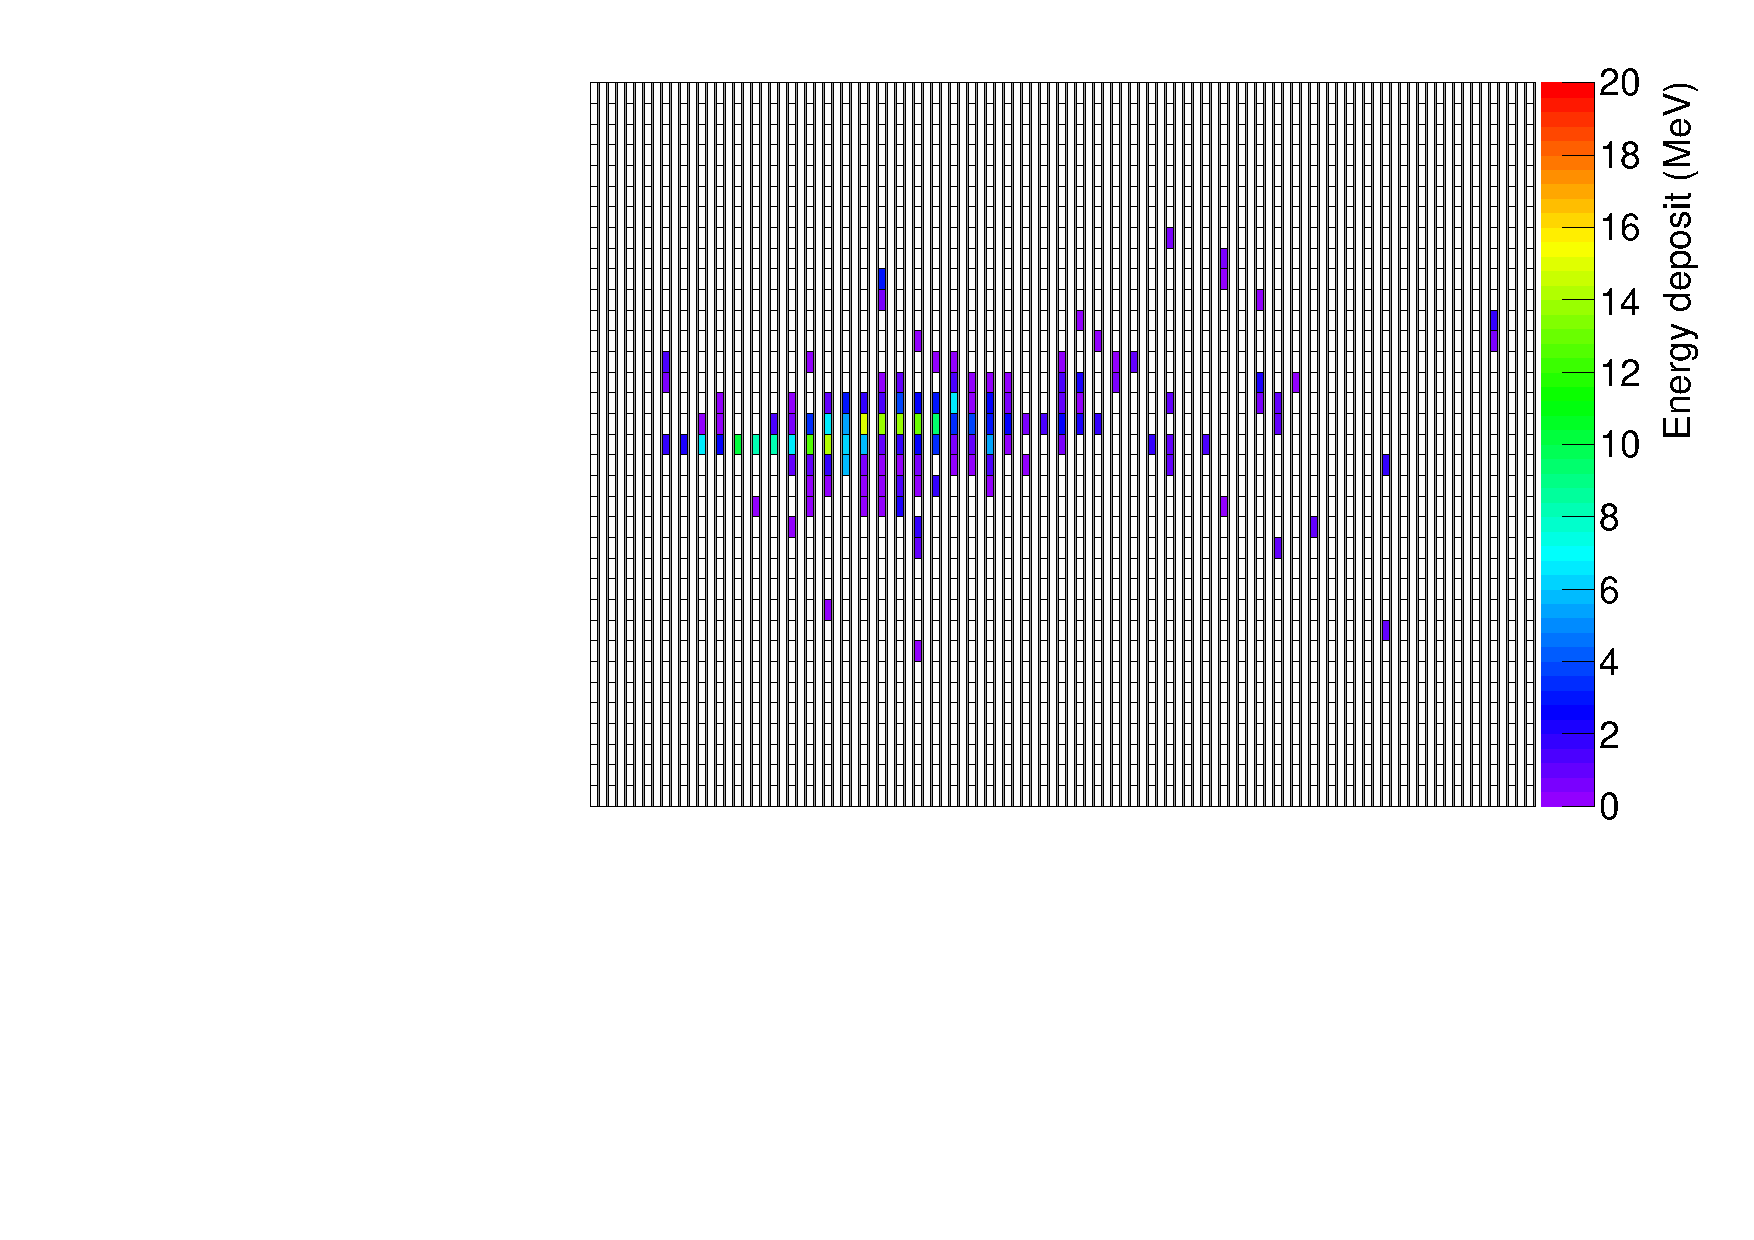
\includegraphics[width=0.48\textwidth]{figures/Fig2_EMShower_YZ.pdf}
\caption{ Event display of simulated energy deposit patterns for a 1-GeV photon entering the calorimeter ($\theta=$~0) in (a) $xz$- and (b) $yz$-planes.}
\label{fig:Evt_Dis}
\end{figure}



The detector response to incident photons was simulated using Geant4 (ver. 4.10.06) with the standard EM sub-packages~\cite{GEANT4}. The normal direction to the detector surface defines the $z$-axis. The photon direction is defines by the polar angle ($\theta$) with respect to the $z$-axis. Figure~\ref{fig:Evt_Dis} illustrates simulated energy deposit patterns in each strip for a 1-GeV photon at a normal incident in $xz$- and $yz$-planes. Each segmented region in Fig.~\ref{fig:Evt_Dis} represents each channel.

\section{Reconstruction of Incident Angles}
\label{sec:res}

Incident angles of photons are reconstructed using XGB~\cite{xgboost:2016}, which maps a feature, dataset of energy deposits in each scintillator strip, into a target variable, the incident angle of a photon. Training data were carefully prepared using the Geant4 simulation such that the input datasets are representative of a detector response of real sampling calorimeters. In order to minimize the bias in the training process related to dataset, the incident angles were uniformly generated at the detector surface in the angular range of 0~$<\theta<$~50$^{\circ}$ and 0~$<\varphi<$~360$^{\circ}$ where $\varphi$ denotes azimuthal angle. The number of training samples is $10^{5}$ considering limited computing resources. To test the reconstruction of incident angles, we generated photons at a fixed incident angle $\theta$, with the known incident energy.

\begin{figure}[!hbt]
\centering
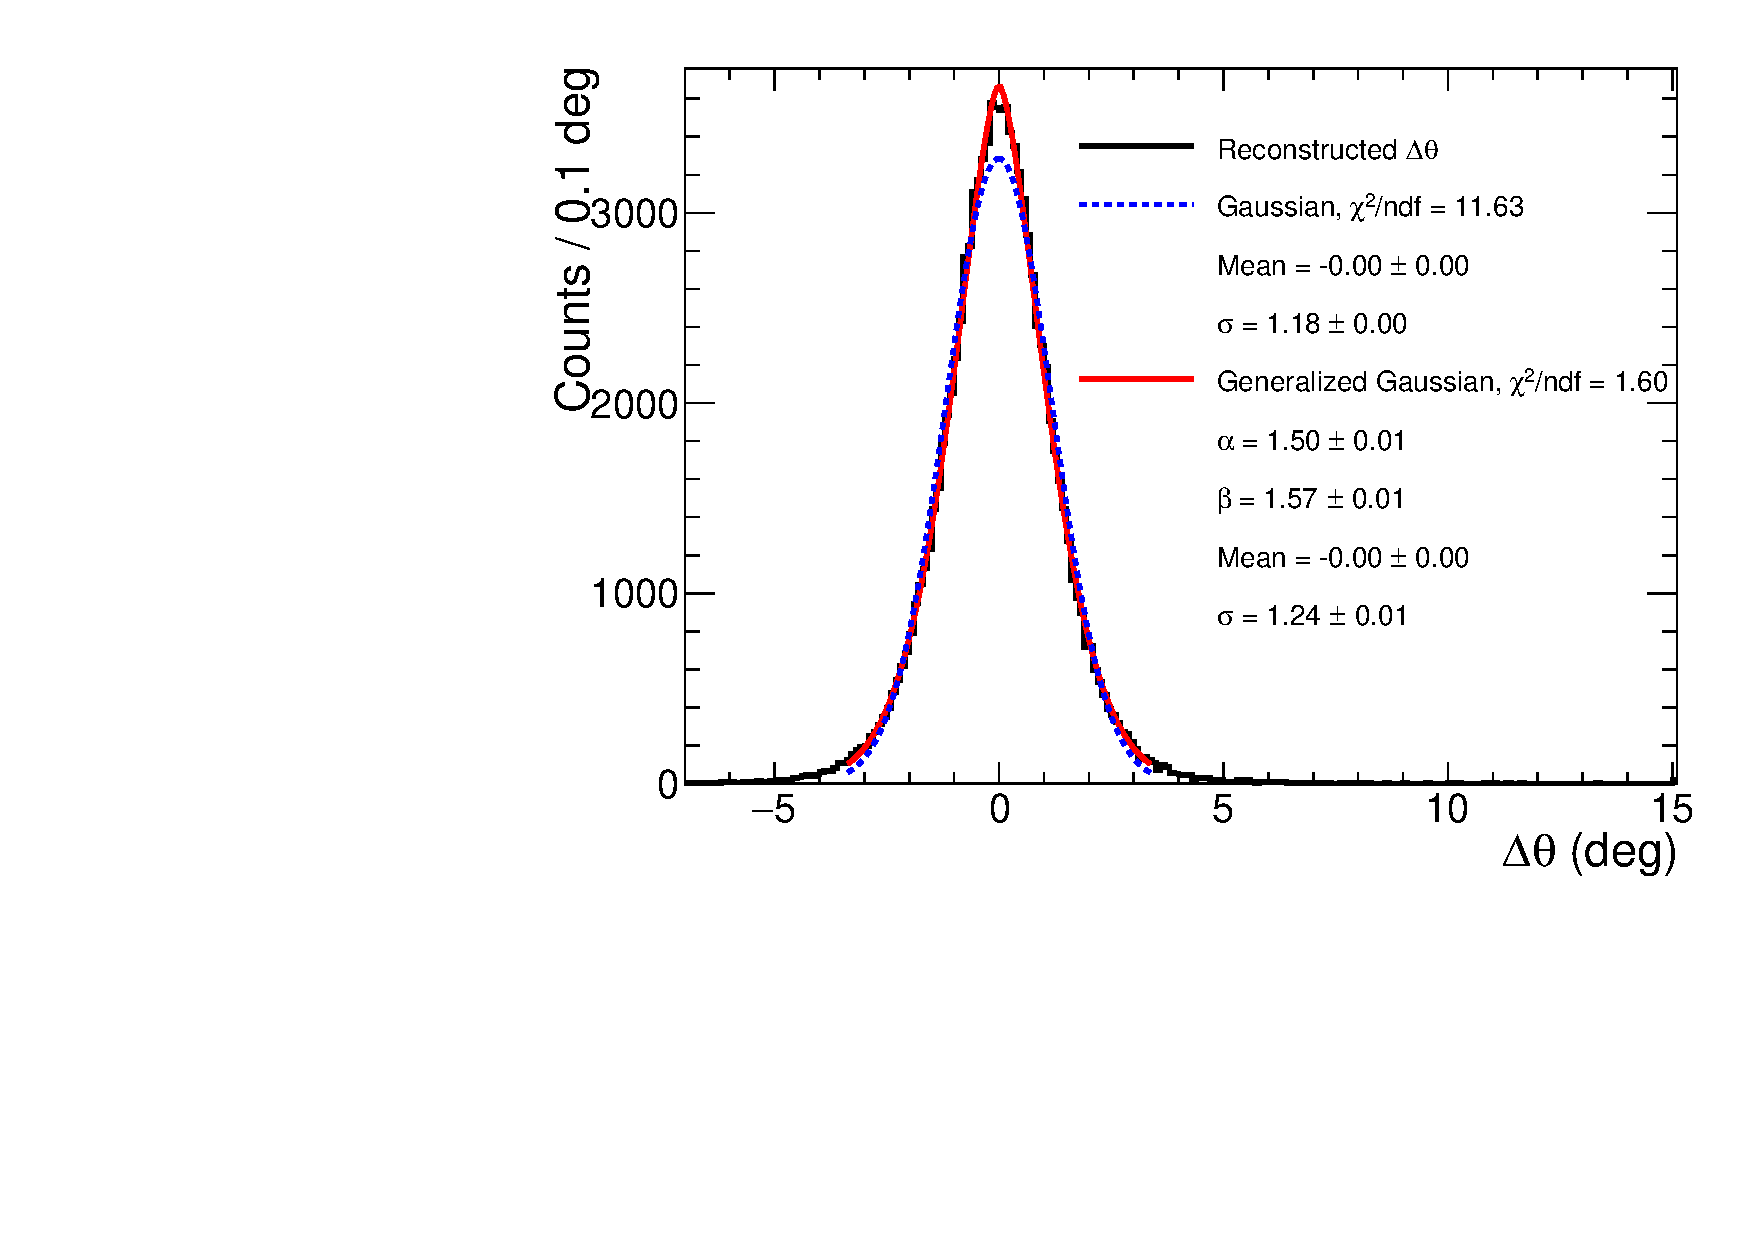
\includegraphics[width=0.7\textwidth]{figures/Fig3_fit_GG.pdf}
\caption{ The relative incident angle for 1-GeV photons generated at $\theta=$~10$^{\circ}$. The distribution is fitted with the Gaussian and the Generalized Gaussian function. The Generalized Gaussian function gives a better result.}
\label{fig:angle_10degree}
\end{figure}

Figure~\ref{fig:angle_10degree} represents a distribution of the relative incident angle ($\Delta\theta$) for 1-GeV photons generated at $\theta=$~10$^{\circ}$. $\Delta\theta$ represents the radial displacement of the reconstructed incident angle from the true incident direction. The central 98\% part of the distribution is fitted with the Gaussian function and the Generalized Gaussian (GG) function~\cite{GGfun}. We tested two functions, the Gaussian and GG to describe the reconstructed angle distribution. The GG function, also known as the generalized error distribution, is expressed as
\begin{eqnarray} 
f(x; \mu, \alpha, \beta) = \frac{\beta}{2 \alpha \Gamma(1/\beta)}e^{-(|x-\mu|/\alpha)^\beta},
\label{eqn:gg}
\end{eqnarray}
where $\mu$ denotes the mean value. Parameters $\alpha$ and $\beta$ determine the scale and shape of the distribution, respectively. Variance of the GG function is given by $\sigma^2 \equiv \alpha^2 \Gamma(3/\beta) / \Gamma(1/\beta)$. The angular resolution of the incident angle reconstruction is defined as $\sigma$.

\begin{figure}[!hbt]
\centering
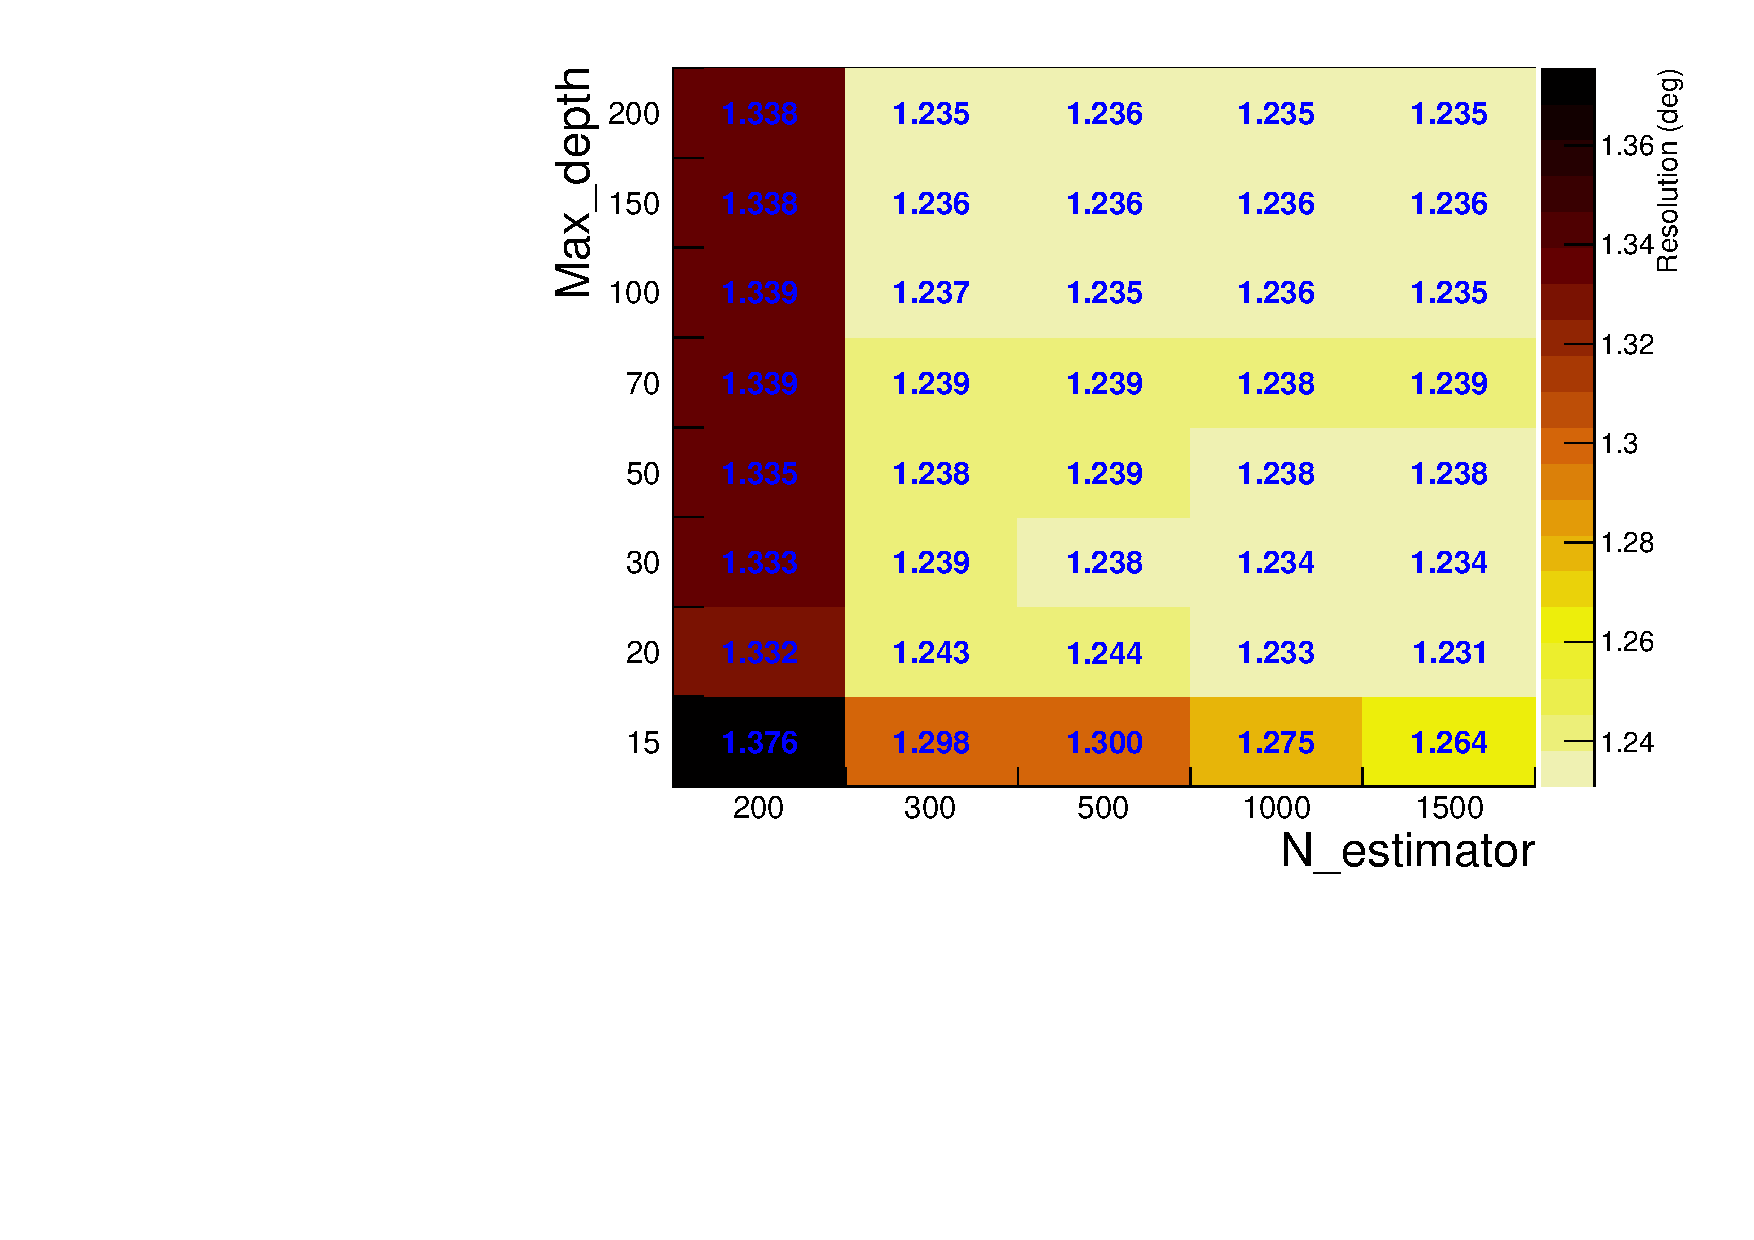
\includegraphics[width=0.69\textwidth]{figures/Fig4_Opt.pdf}
\caption{Angular resolutions are displayed in terms of combination of N\_estimators and Max. depth. The best angular resolution is obtained with N\_estimators~=~300 and Max. depth~=~100. }
\label{fig:par_scan}
\end{figure}

Since the performance of angle reconstruction of the XGB depends on hyperparameters, we scanned evaluated angular resolution by changing the hyperparameters. As there are correlations among the hyperparameters, the scanning process was performed in five dimensional space for all possible combinations. As an example, figure 4 shows the test results with N\_estimators and Max. depth. N\_estimators defines the maximum allowed number of decision trees to be developed, and the Max. depth defines the complexity of the structure of decision trees. We searched for the hyperparameter combination that generated the best angular resolution. As a result, N\_estimators and Max. depth are set to 300 and 100, respectively. Similar scans were also performed for different hyperparameters, Subsample, Learning rate, and Gamma. Subsample controls the fraction of total event samples for each boosting procedure, Learning rate weights a decision tree to be added onto the current model, and Gamma regulates the evaluation of each decision tree. Table~\ref{tab:XgbPar} summarizes optimizes set of hyperparameters which was used for further studies. During the optimization process, the fraction of the tail that is not well described by the GG function is around 2\%.

\begin{table}[hbt!]{\small
\centering
\caption{Hyperparameters of the XGB model}
\begin{tabular}{cccc}
\hline 
Parameter & Function & Default value & Used value \\ \hline 
N\_estimators & The number of decision trees & N.A. & 300 \\  
Max. depth & Possible maximum depth of tree structure & 6 & 100 \\ 
Subsample & Fraction of total data used for a single decision & 1 & 0.8 \\ 
Learning rate & Step length for calculation & 0.3 & 0.02 \\ 
Gamma & Requirement on minimum loss function & 0 & 0 \\ 
\hline
\end{tabular}
\label{tab:XgbPar}
}\end{table}

\begin{figure}[!hbt]
\centering
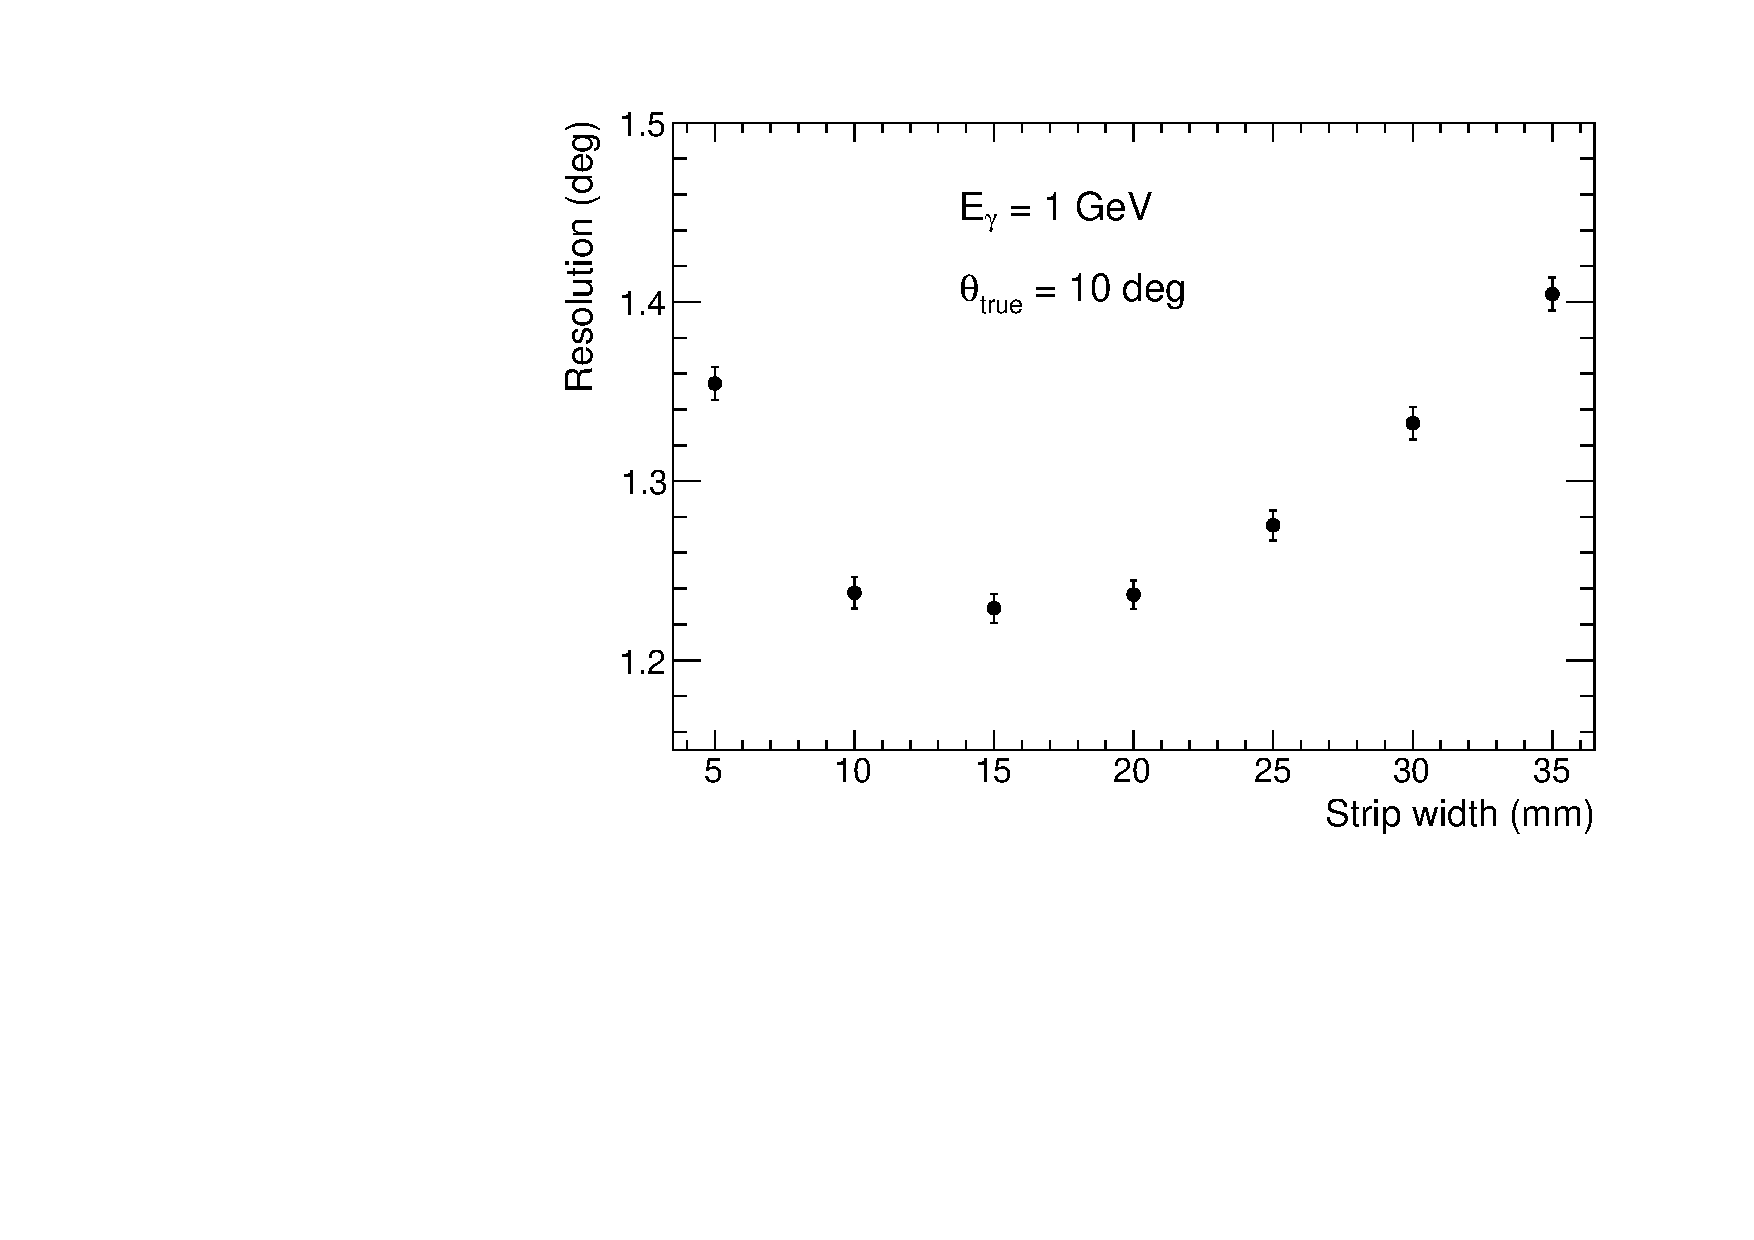
\includegraphics[width=0.58\textwidth]{figures/Fig5_width.pdf}
\caption{ Angular resolutions are deduced in terms of the strip width for 1-GeV photons at $\theta=$~10$^{\circ}$ }
\label{fig:angle_reco_width}
\end{figure}

Angular resolutions were deduced by varying strip widths from 5 mm to 35 mm as shown in Fig.~\ref{fig:angle_reco_width}.  The narrower the strip width is used, the larger the size of the features becomes. As a result, the performance of the angle reconstruction decreases. On the other hand, the wider strips hardly provide the detailed information on the EM shower. The 15-mm-wide strips yield good angular resolution of 1.23~$\pm$~0.01$^{\circ}$.

\begin{figure}[!hbt]
\centering
\stackinset{c}{0.cm}{b}{-0.4cm}{(a)}{
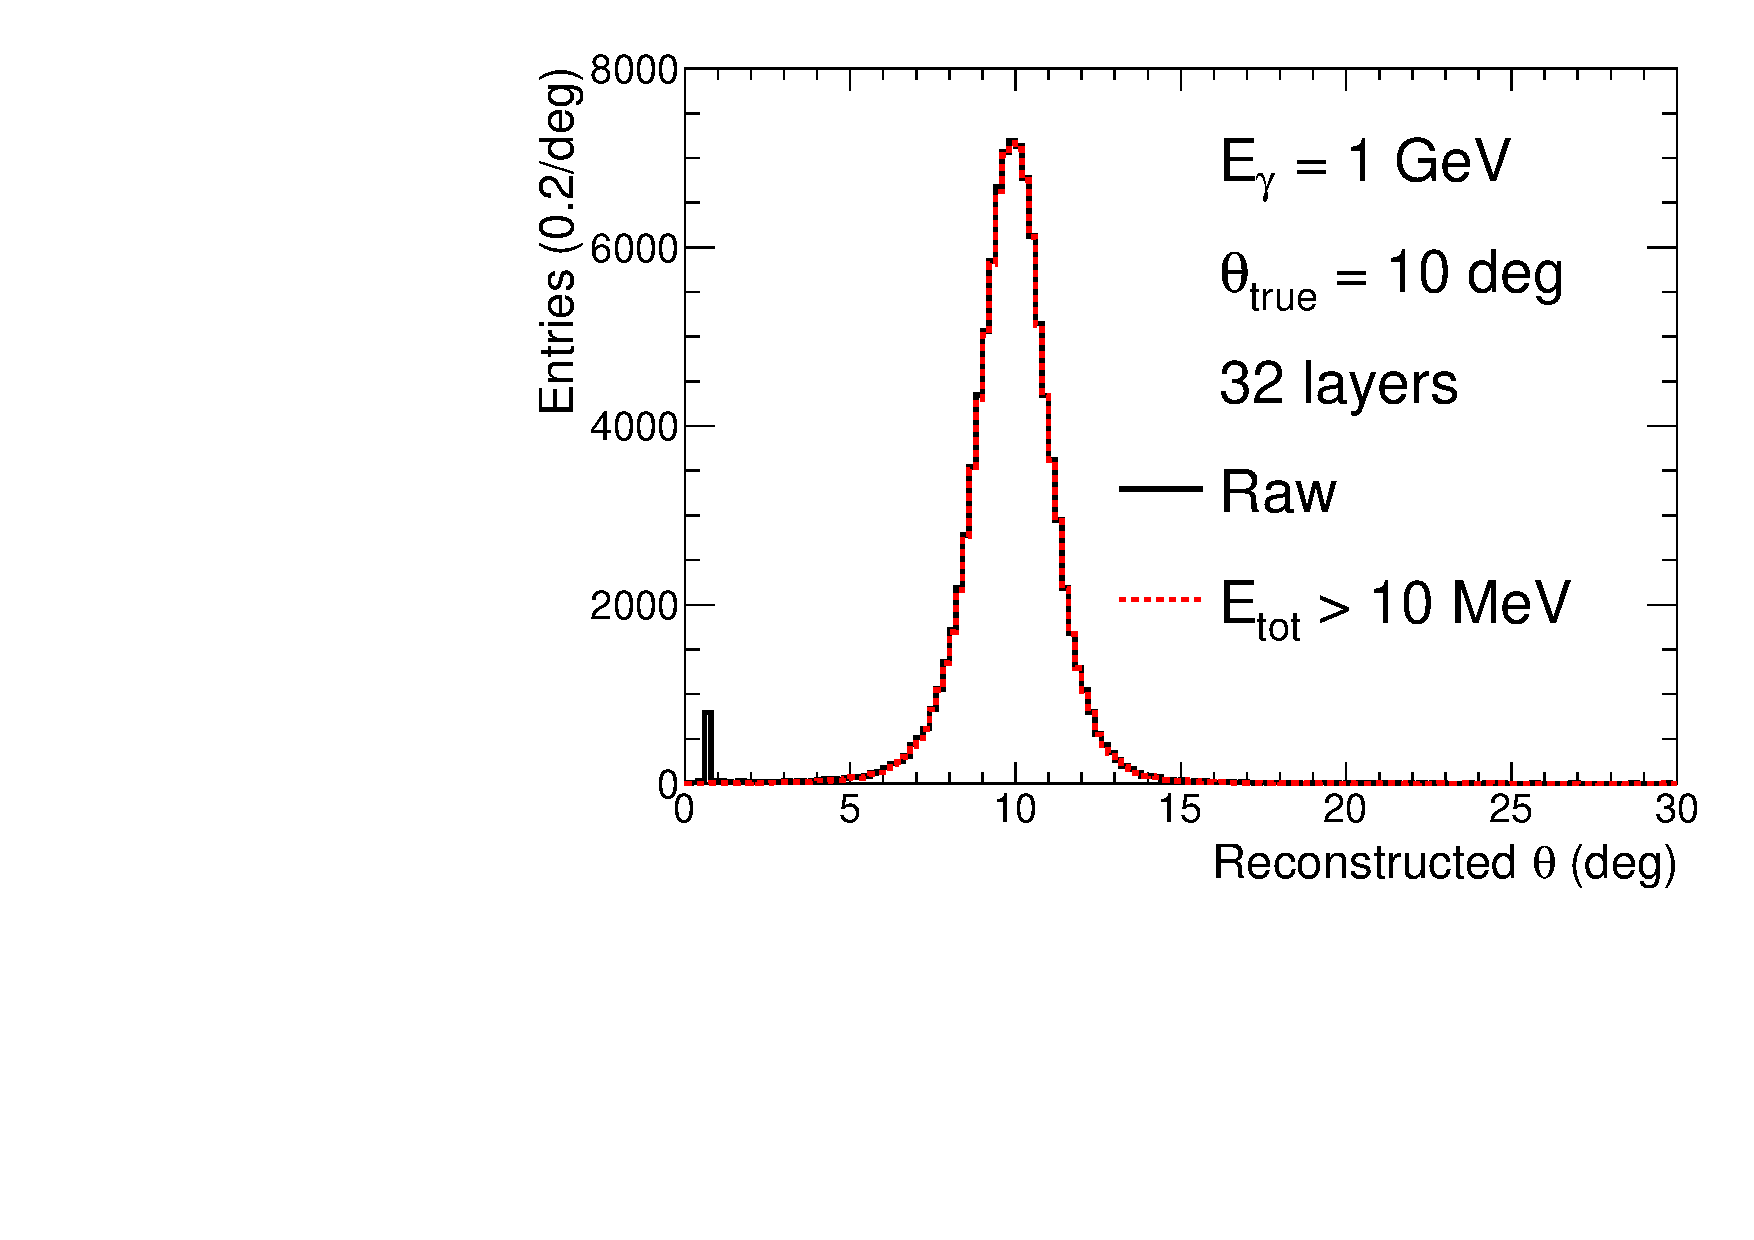
\includegraphics[width=0.48\textwidth]{figures/Fig6_layer_comp.pdf}
}\stackinset{c}{0.cm}{b}{-0.4cm}{(b)}{ 
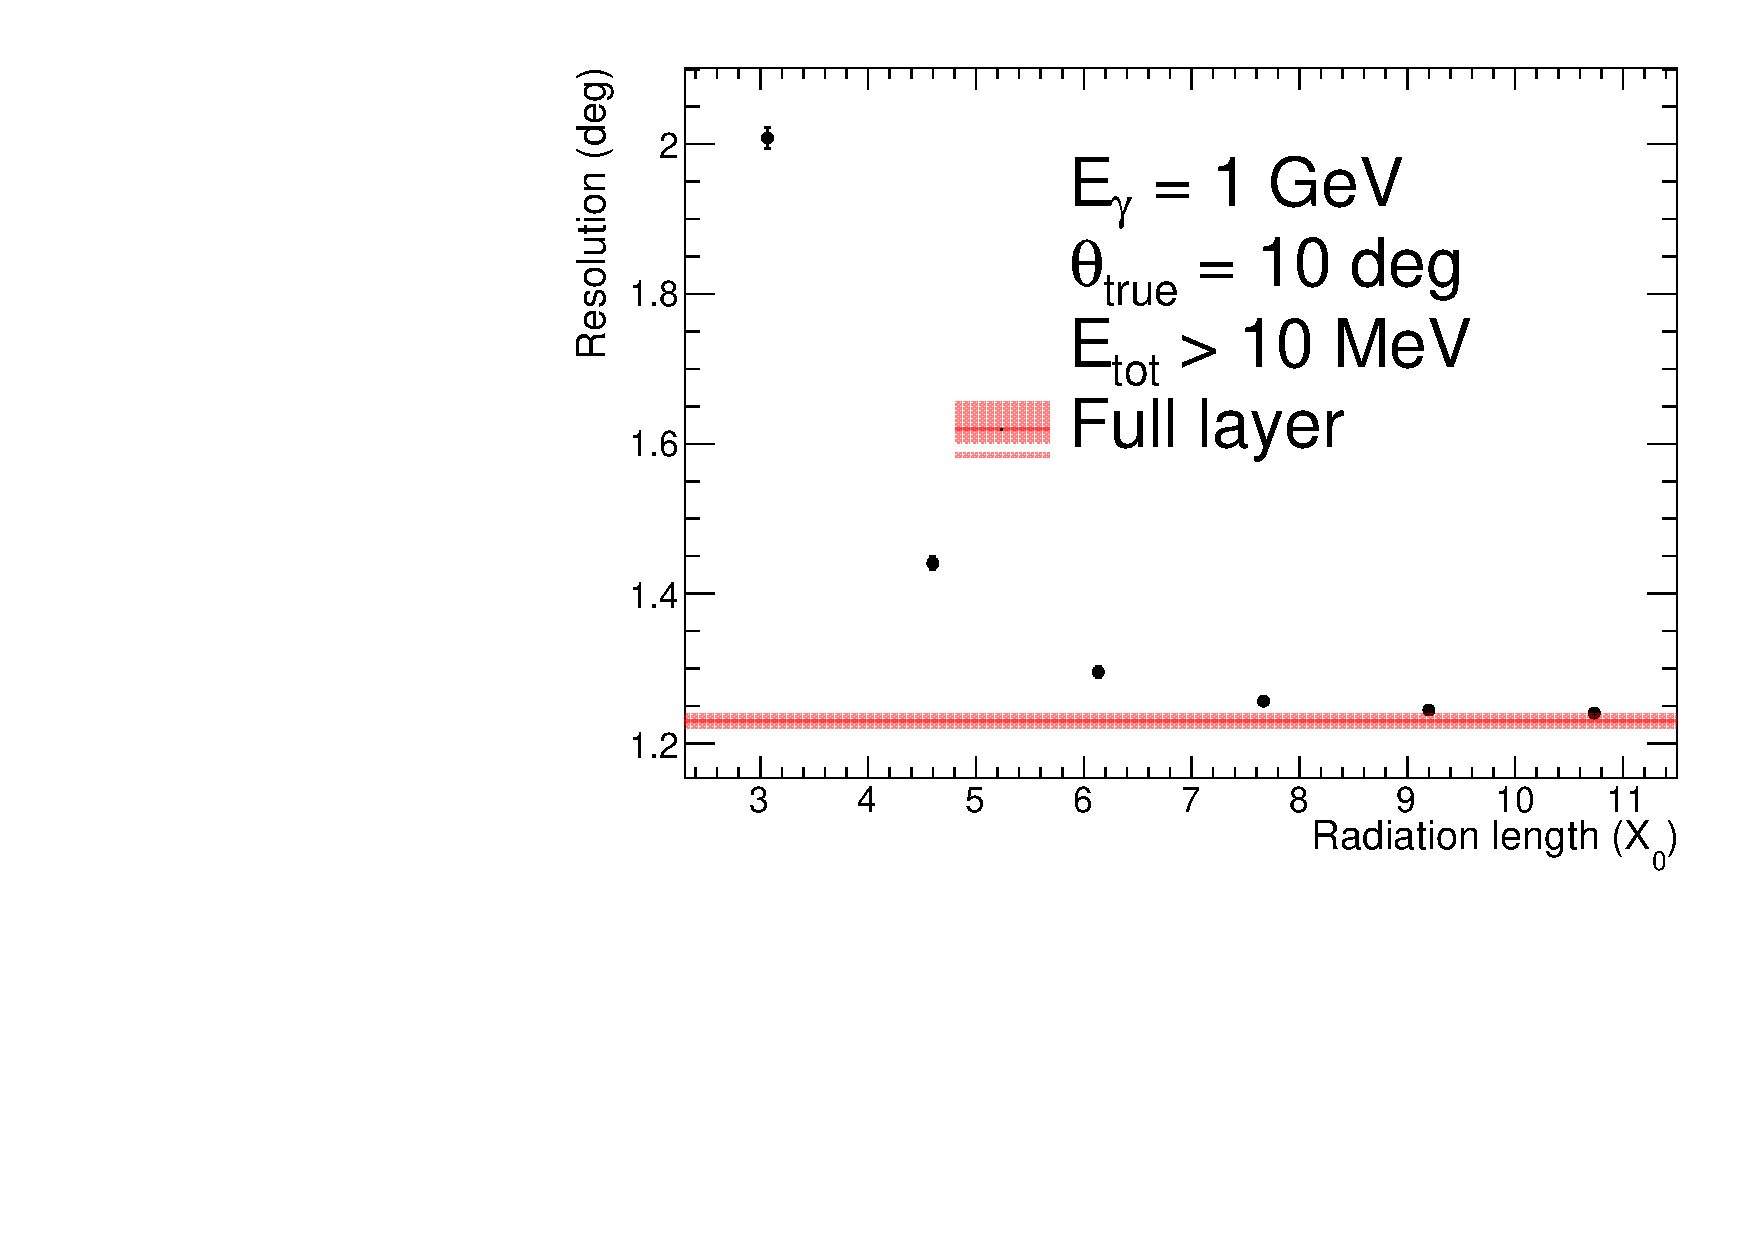
\includegraphics[width=0.48\textwidth]{figures/Fig6_nlayer.pdf}
}
\caption{ (a) Reconstructed polar angles ($\theta$) for 1-GeV photons at $\theta=$~10$^{\circ}$. Red histogram represents the polar angle distribution by requiring $E_{\rm{tot}}>$~10~MeV. (b) Angular resolution as a function of radiation length ($X_{0}$).}
\label{fig:angle_reco_layer}
\end{figure}

Focusing only on the angle reconstruction, we design the detector towards the smallest number of layers. Figure~\ref{fig:angle_reco_layer} (a) shows reconstructed angles using the front 32 layers of the detector, which correspond to 6.2$X_{0}$, for 1-GeV photons. A fraction of photons failed to be reconstructed due to insufficient information caused by deeply penetrating photons without shower generation. The failed events are represented as a delta function near 0, and such events are removed by requiring the total energy deposit to be larger than 10~MeV, 1\% of the incident energy. The angular resolution with the front layer is estimated to be 1.30~$\pm$~0.01$^{\circ}$ while 1.9\% of photons fail to be reconstructed.

\begin{figure}[!hbt]
\centering
\stackinset{c}{0.cm}{b}{-0.4cm}{(a)}{
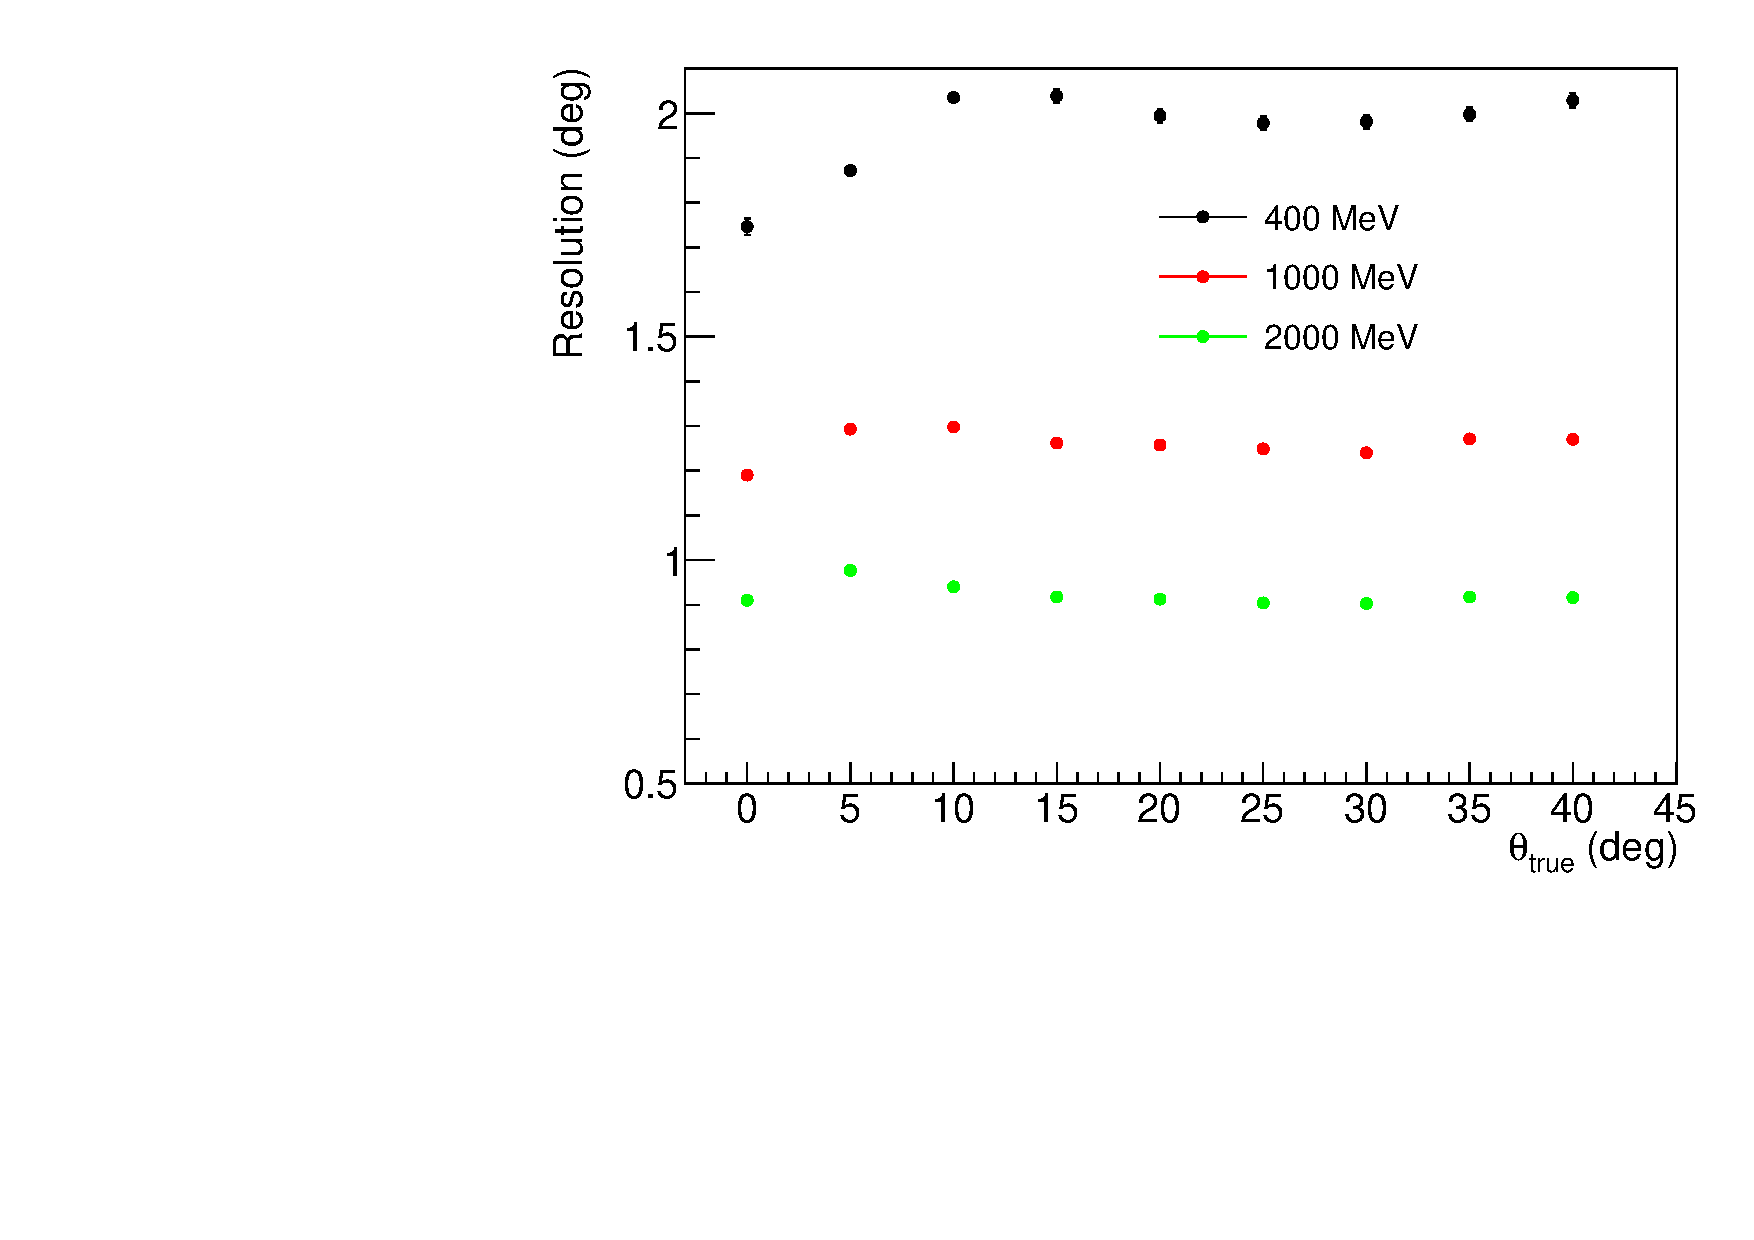
\includegraphics[width=0.44\textwidth]{figures/Fig7_res_ene.pdf}
}\stackinset{c}{0.cm}{b}{-0.4cm}{(b)}{
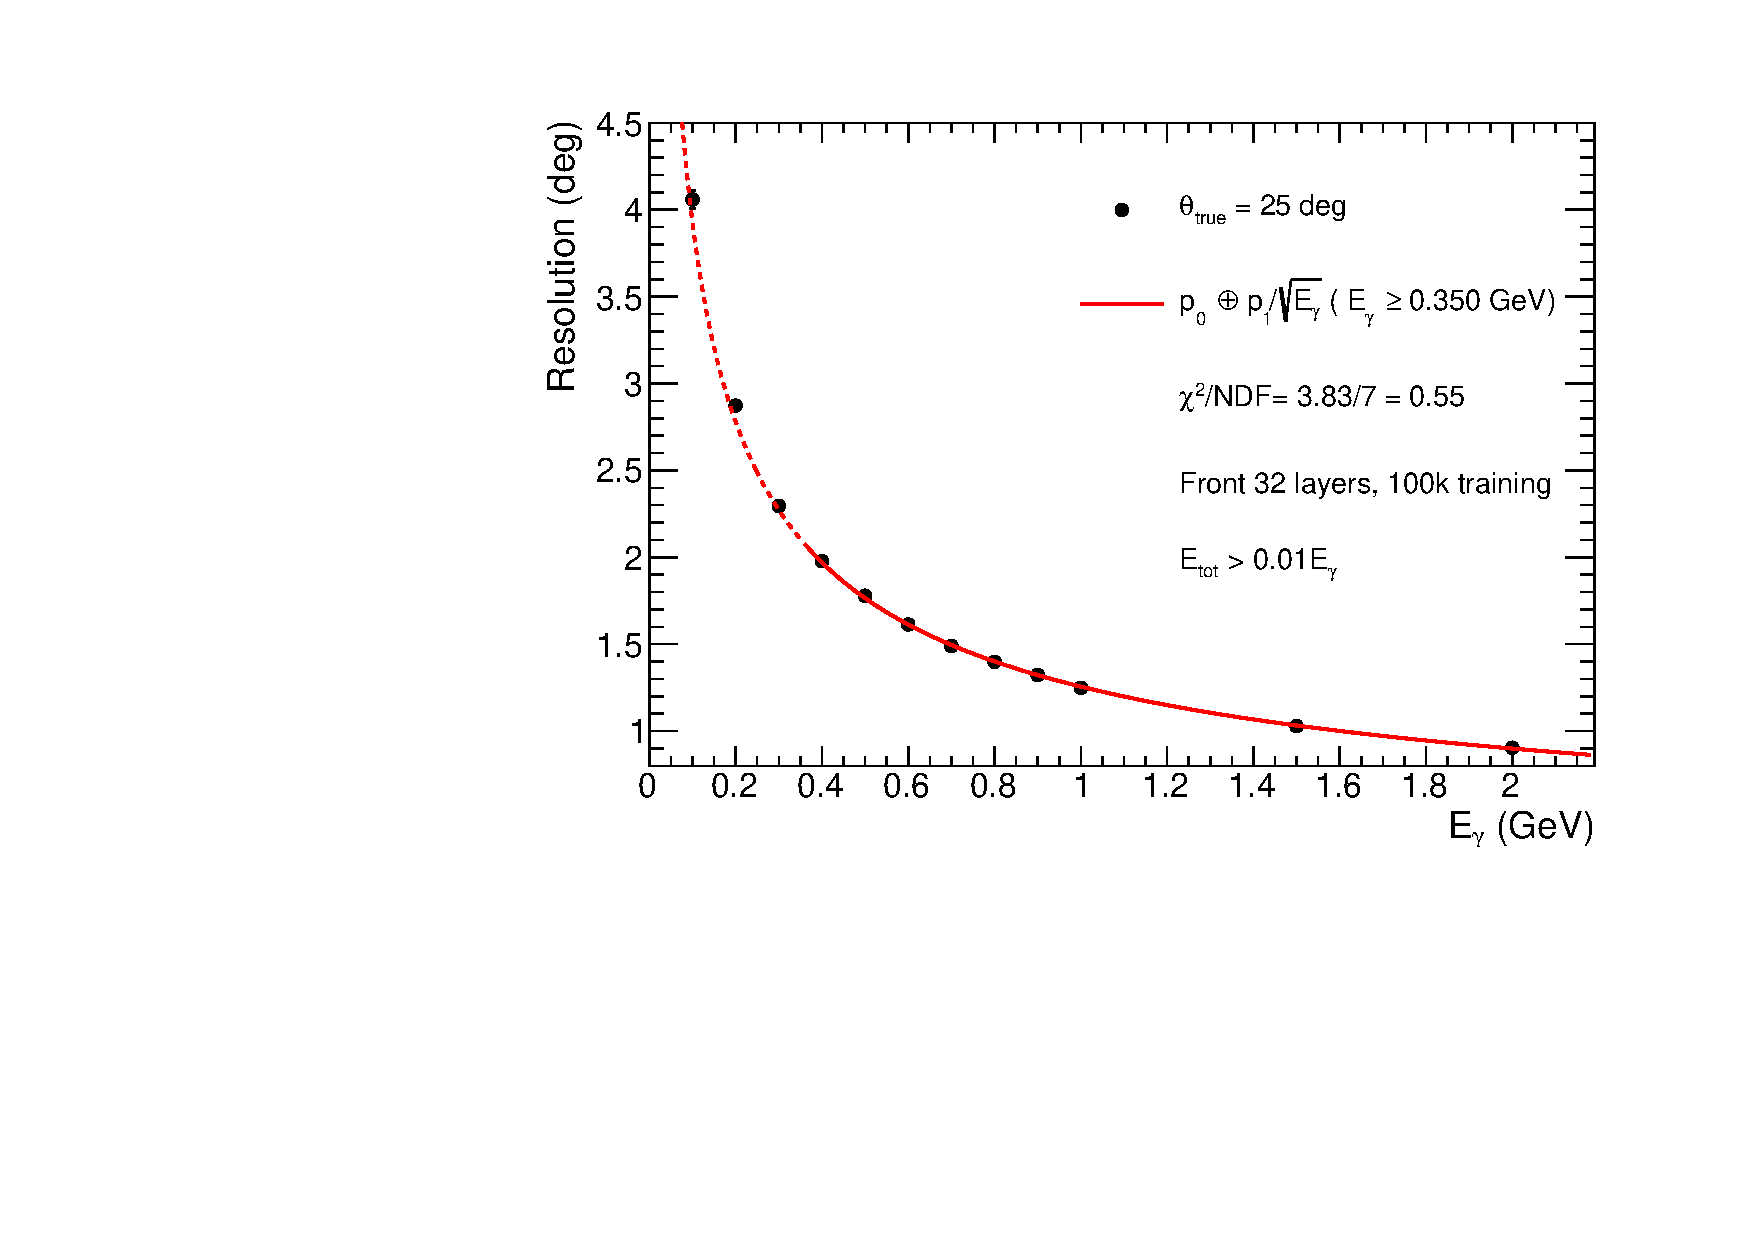
\includegraphics[width=0.44\textwidth]{figures/Fig7_Fit_eres_1.pdf}
}
\caption{ Angular resolutions as functions of the incident angle for different incident energies (a) and the incident energy for $\theta=$~25$^{\circ}$, which is fitted with $p_{0} \oplus p_{1}/\sqrt{E_{\gamma}(\mathrm{GeV})}$ (b) }
\label{fig:angle_reco_dep_gr}
\end{figure}

Figure~\ref{fig:angle_reco_dep_gr} (a) shows the angular resolution as a function of the incident angle for different incident energies ($E_{\gamma}$). The angular resolution does not depend on the incident angle for high incident energy. On the other hand, the angular resolution changes significantly for low incident energy at small incident angle. Figure~\ref{fig:angle_reco_dep_gr} (b) shows the angular resolution as a function of the incident photon energy at $\theta=$~25$^{\circ}$. The angular resolutions fit to a function of $p_{0} \oplus p_{1}/\sqrt{E_{\gamma}(\mathrm{GeV})}$, where $p_{0}$ and $p_{1}$ represent an energy independent and energy dependent contribution, respectively.

\begin{figure}[!hbt]
\centering
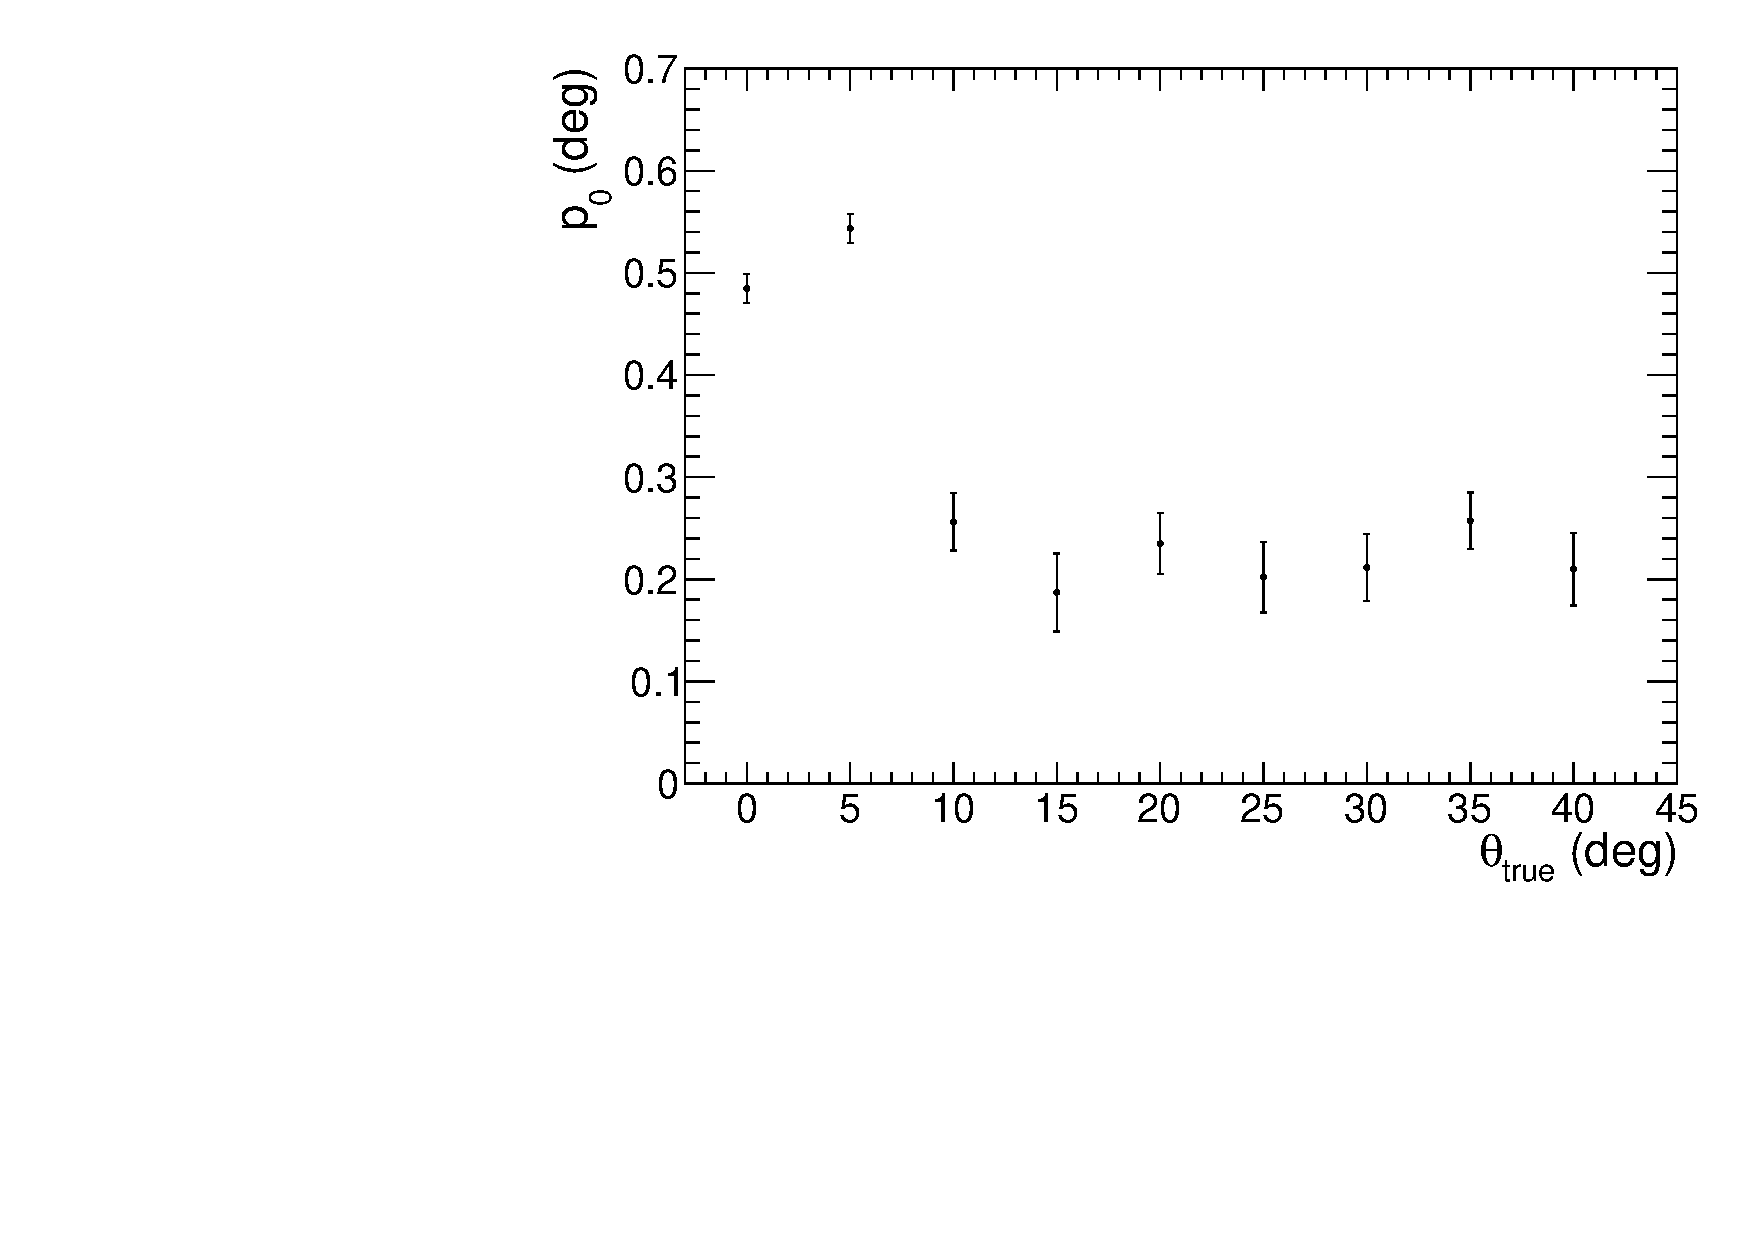
\includegraphics[width=0.44\textwidth]{figures/Fig7_p0.pdf}
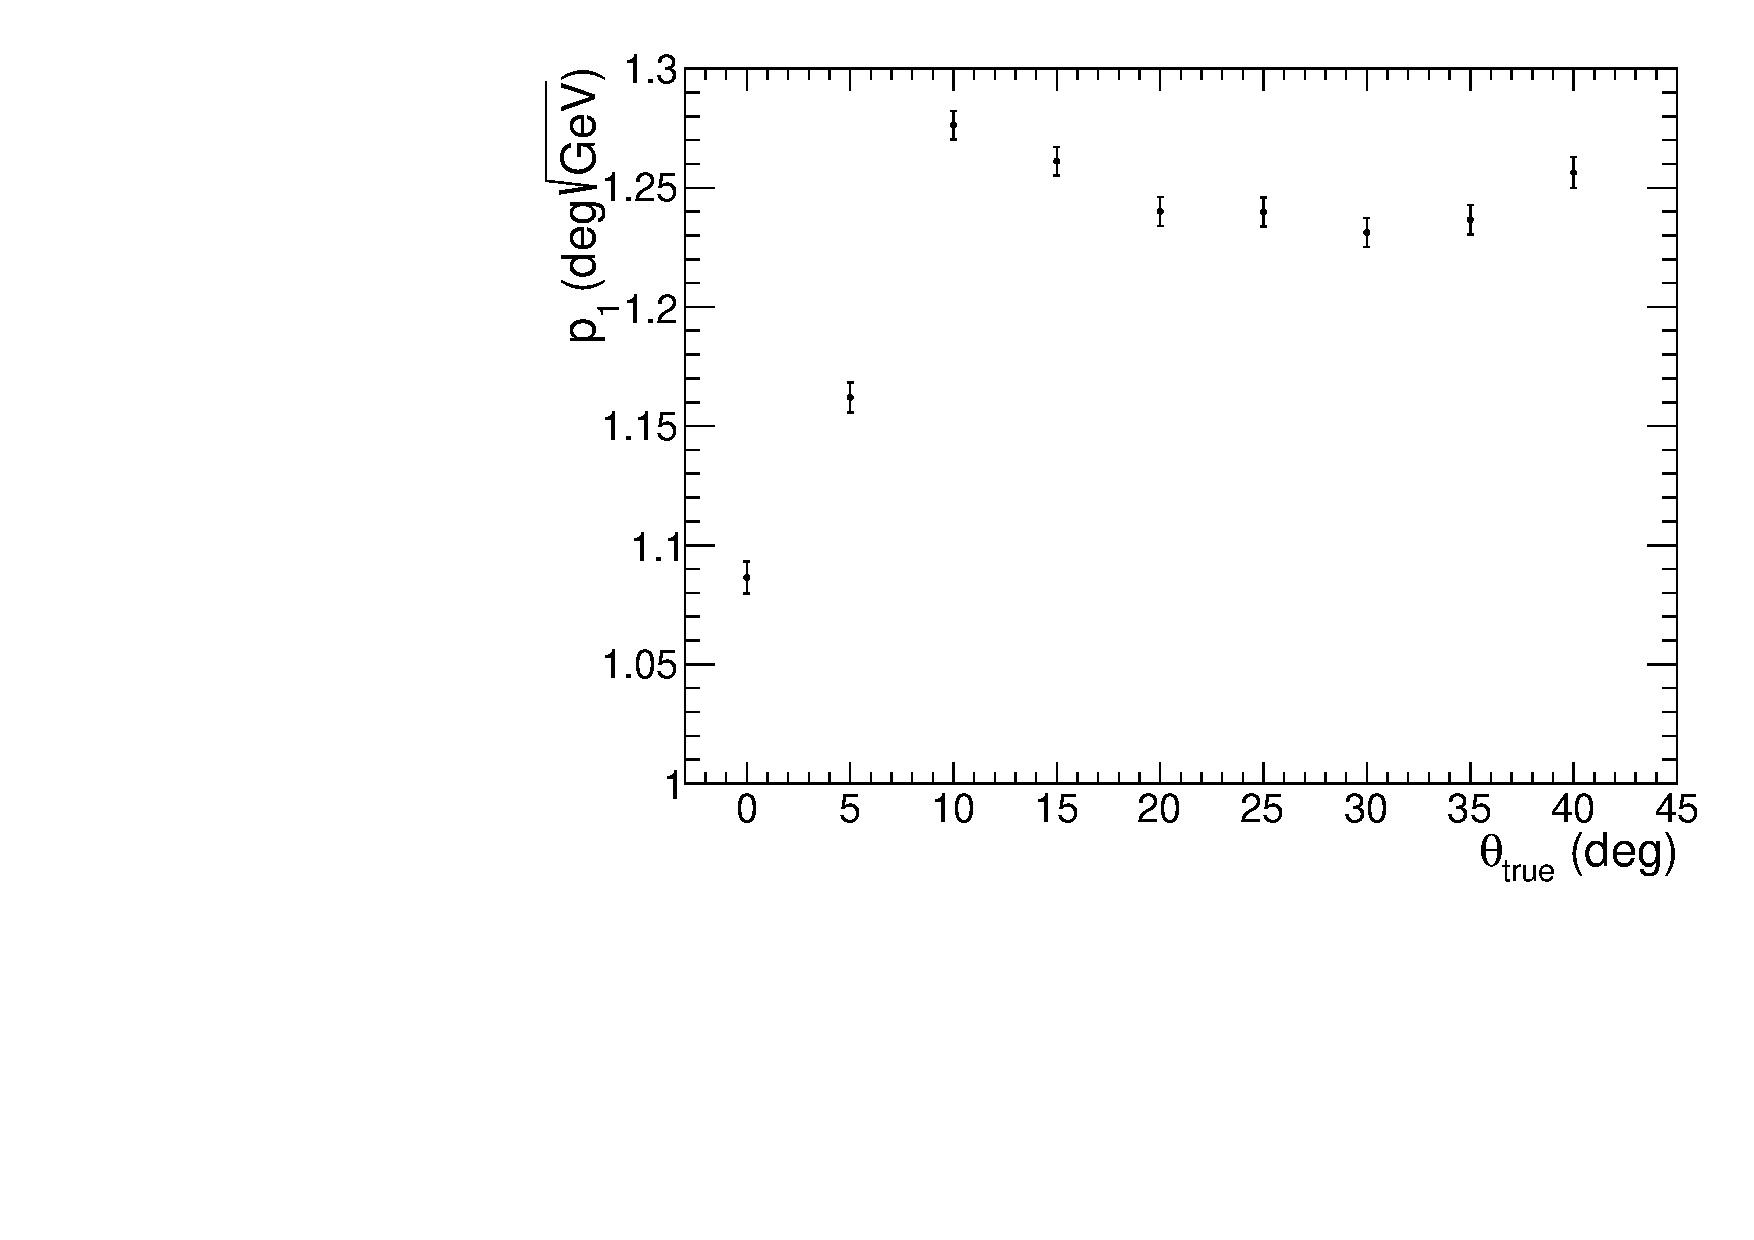
\includegraphics[width=0.44\textwidth]{figures/Fig7_p1.pdf}
\caption{ $p_{0}$ and $p_{1}$ as a function of the incident angle }
\label{fig:res_edep}
\end{figure}

Figure~\ref{fig:res_edep} shows estimated $p_{0}$ and $p_{1}$ as a function of the incident angle. $p_{0}$ and $p_{1}$ are estimated to be 0.24$^{\circ}$ and 1.24$^{\circ}$, respectively in average for $\theta>$~10$^{\circ}$. For small $\theta$, $p_{1}$ is smaller than larger $\theta$ from the fact that the angular resolution is largely dependent on the incident angle for the low incident energy while opposite trend can be seen for $p_{0}$.

\begin{figure}[!hbt]
\centering
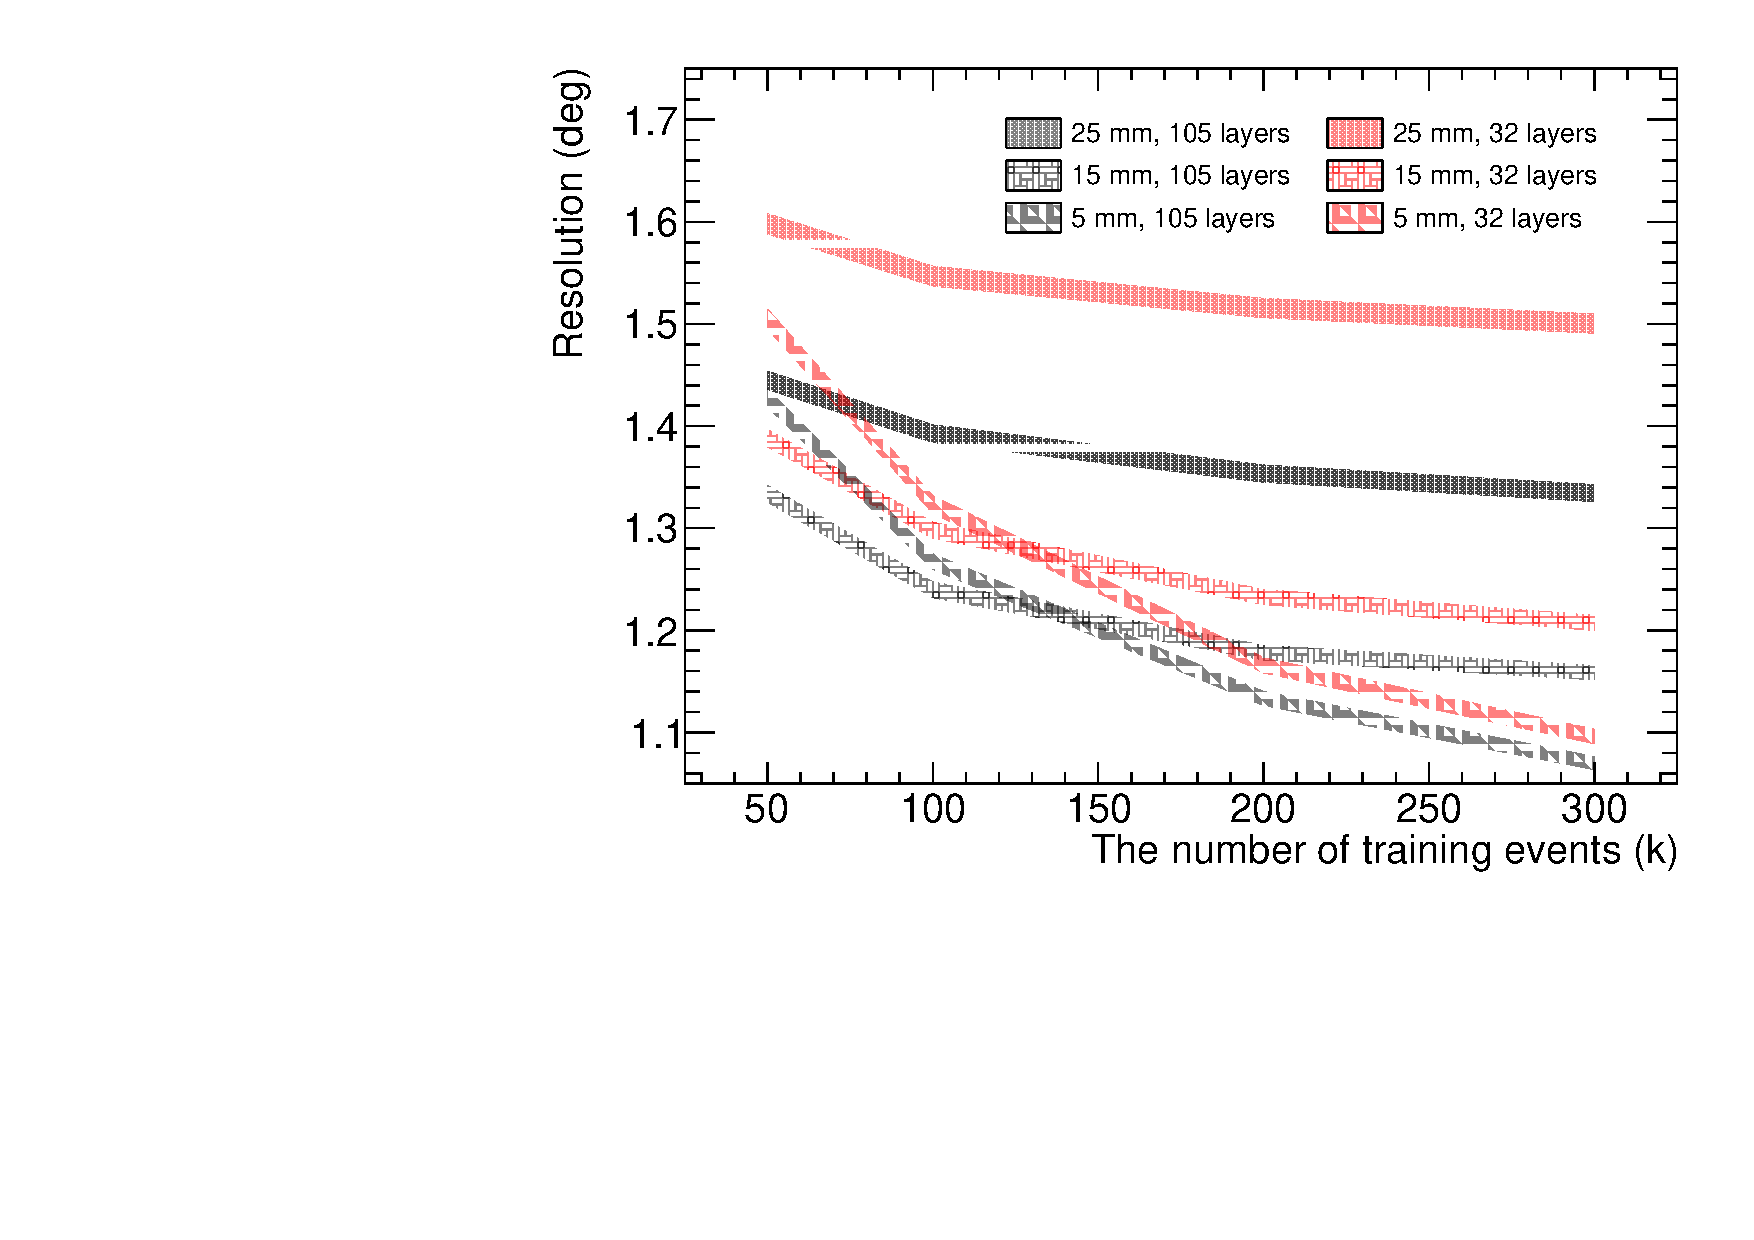
\includegraphics[width=0.6\textwidth]{figures/Fig8_nsample.pdf}
\caption{ The angular resolution for 1-GeV photons at $\theta=$~10$^{\circ}$ as a function of the number of training samples with different strip widths using the first 32 layers or the full layers. }
\label{fig:multi-parameter}
\end{figure}

Figure~\ref{fig:multi-parameter} shows the angular resolution with different numbers of training samples for different detector configurations. All configurations show improvement in the angular resolution with increasing training samples, which means that the maturity of the machine learning is an important factor on the angle reconstruction. The angular resolution with 5-mm-wide scintillator strips is the most rapidly improved with the increasing number of training events. That is, the required training events should be large enough to correlate the larger number of features. Considering limited computing resources, the configuration of 32 layers and the 15-mm-wide strip with $10^{5}$ training events was chosen for training the XGB model. The training result differs by only 0.2$^{\circ}$ from the setup with full layers, 5-mm-wide strips, and $5\times10^{5}$ training events.
 
\section{SUMMARY}
\label{sec:sum}

We report simulation results on the incident angle reconstruction of EM sampling calorimeters with photons in the range of 0.1 to 2~GeV. In order to improve the angular resolution, we tune the hyperparameters of the XGBoost taking into account correlating effects among them.

In terms of the detector configuration, strips having narrower width provide better angular resolution using finely measured EM shower with the assumption that the training is fully conducted. On the other hand, the configuration with smaller strip width causes larger feature size, which negatively affects the training depending on the quantity of training data. We may optimize the angular resolution considering two competing effects from the strip width and the quantity of training data. We dedicate front layers of the detector to reconstructing the incident angle. We obtain the angular resolution of 1.30~$\pm$~0.01$^{\circ}$ with 32 layers (6.2$X_{0}$) of 15-mm-wide strips, which becomes worse by only 0.1$^{\circ}$ compared to that of the full layers (20$X_{0}$) in case of $10^{5}$ training samples. 

The angular resolution depends on photon’s incident energy, where the dependence is expressed as $p_{0} \oplus p_{1}/\sqrt{E_{\gamma}}$. Except for small incident angles ($\theta<$~15~deg), the two parameters do not significantly change up to 40 degrees and the dependence is estimated to be 0.24 $\oplus$ 1.24$^{\circ}/\sqrt{E_{\gamma}}$. 

\label{sec:con}

%\pagebreak


\section*{Acknowledgment}
This paper was supported by the National Research Foundation of Korea (NRF) grants funded by the Korea government (MIST) (2019R1A2C1084552, \\ 2022R1A5A1030700, and 2020R1A3B2079993)

\begin{thebibliography}{99}
 
\bibitem{KOTO:MB}
Y. Tajima {\it et al.}, Nucl. Instrum. Meth. A 592, 261 (2008).

\bibitem{CMS:EMCAL}
Giovanni Mazza {\it et al.} (CMS Collaboration), Nucl. Instrum. Meth. A 958 (2020)

\bibitem{BELLE:EMCAL}
K. Miyabayashi {\it et al.}, JINST 9 (2014) 09, P09011

\bibitem{Murayama:2020mcp}
R. Murayama {\it et al.}, Nucl. Instrum. Meth. A 953 (2020) 
 
\bibitem{trk:ref}
O. Adriani {\it et al.}, Nucl. Instrum. Meth. A 854 (2017) 

\bibitem{xgboost:2016}
C. Tianqi {\it et al.}, 
{\it Proceedings of the 22nd ACM SIGKDD International Conference on Knowledge Discovery and Data Mining},
(2016) 785.

\bibitem{GGfun}
D. Gonzalez {\it et al.}, IEEE Trans. Image Processing. 4, 485 (2007)

\bibitem{GEANT4}
S. Agostinelli {\it et al.},  Nucl. Instr. and Meth. A {\bf 506} (2003) 250.

\end{thebibliography}

%\section*{Acknowledgement}
%This paper was supported by the National Research Foundation of Korea (NRF) grants funded by the Korea government (MIST) (2019R1A2C1084552 and \\ 2020R1A3B2079993).

%\bibliographystyle{elsarticle-num}
%\bibliography{paper.bib}

%\printbibliography

\end{document}
